\documentclass[12pt, oneside]{article} 
\usepackage[left=15mm, right=15mm, top=10mm]{geometry}
\usepackage{graphicx}
\usepackage{url}
\usepackage{multicol}
\usepackage{hyperref}
\usepackage{float}

\begin{document}
\title{Techniques d'attaque - DVWA}
\author{Tristan BILOT, Nora DELFAU, Enzar SALEMI, Madushan THAMBITHURAI\\EPITA}
\date{20 Juillet 2021}
\maketitle

\begin{abstract}
L'objectif de ce TP sera d'exploiter différentes vulnérabilités de difficultés variées en utilisant comme cible le site d'entraînement DVWA. Il s'agira ainsi de s'exercer cette fois-ci sur les vulnérabilités web les plus connues. Plusieurs outils seront utilisés dont hydra, burp et sqlmap.
\end{abstract}

\section{Attaque de l'authentification par dictionnaire}
Tout d'abord, en analysant le code de la page de connexion, nous observons que la connexion s'effectue par un simple formulaire, faisant transiter les credentials d'authentification par méthode POST. Il est alors possible de forger des requêtes POST en masse afin de les envoyer au serveur chargé de l'authentification, si aucun mécanisme de bloquage n'est implémenté.

\begin{figure}[H]
\centering
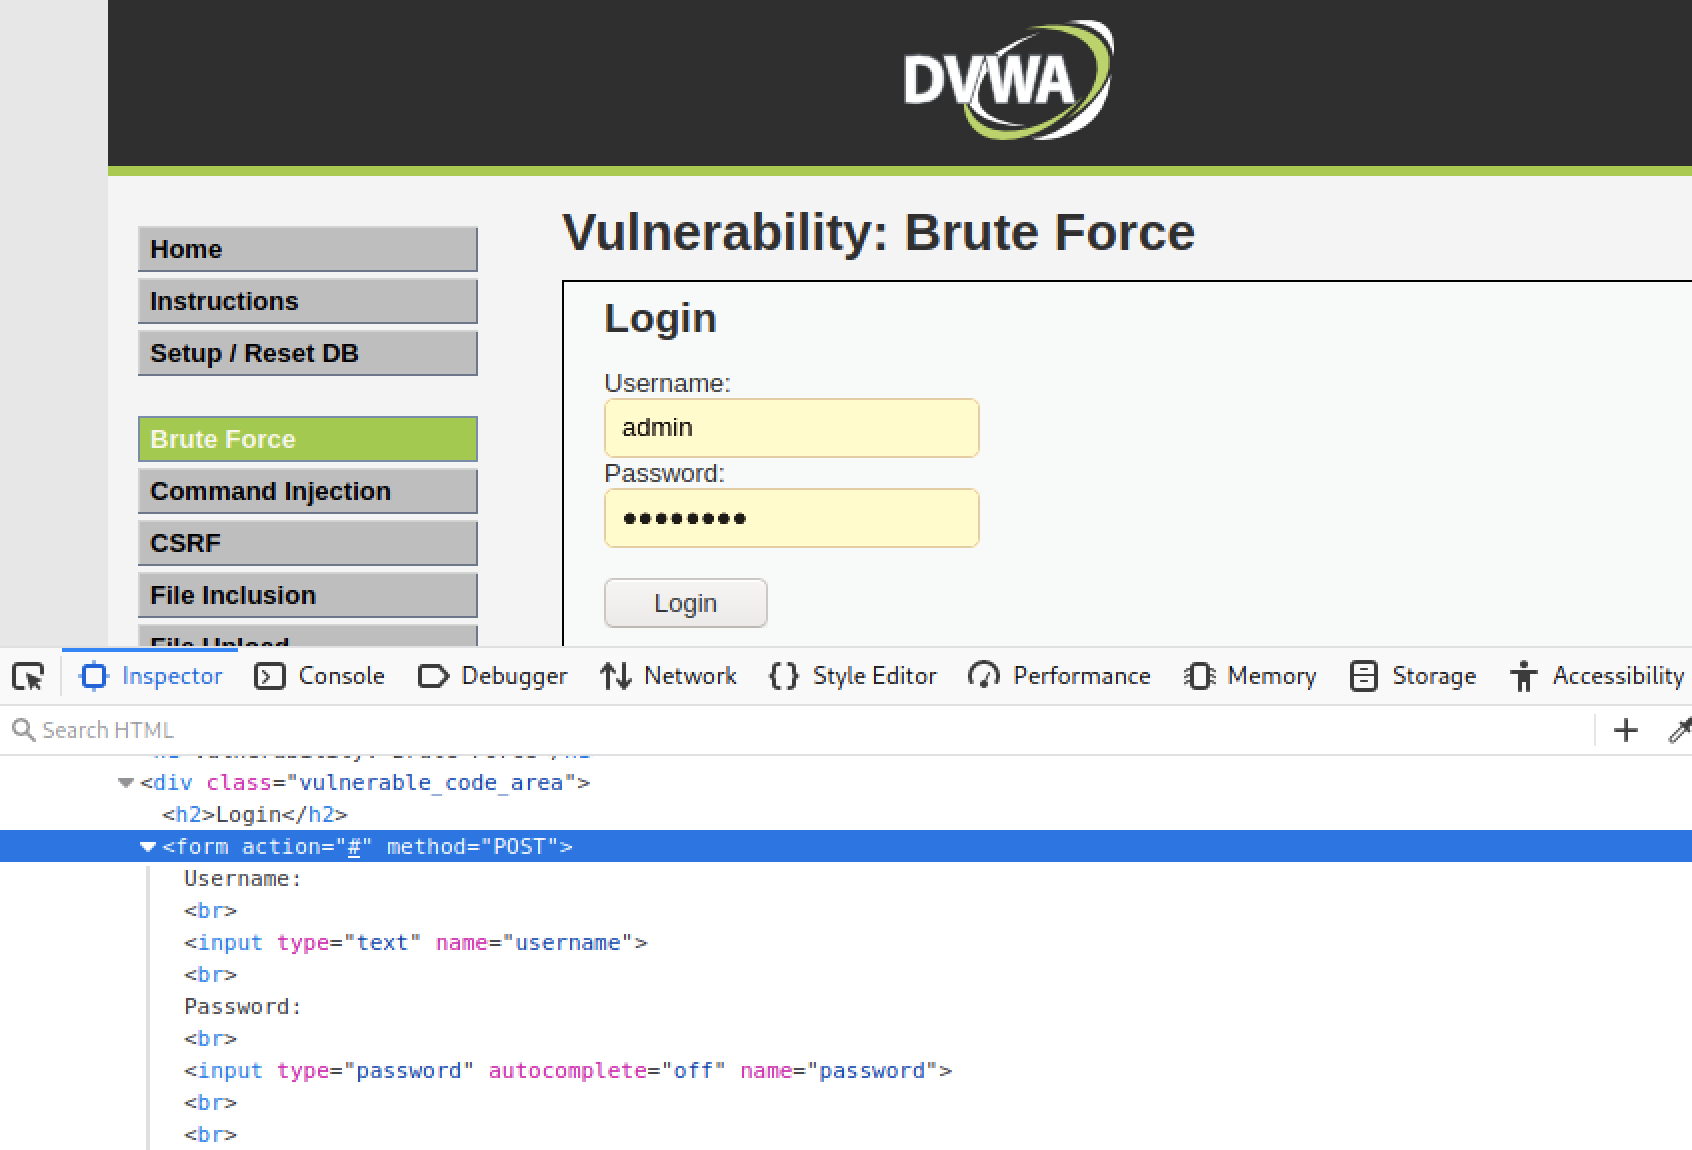
\includegraphics[scale=0.4]{1}
\caption{Formulaire de connexion POST}
\end{figure}

Il est constaté qu'un delay de 15 minutes est activé après une tentative de connexion échouée. Cependant, les credentials utilisés pour la connexion ont été découvert aisément puisqu'il s'agit des mêmes identifiants que ceux de la connexion au site DVWA: admin/password.
Nous allons tout de même procéder à une attaque par dictionnaire afin de s'immerger dans un cas qui pourrait être plus proche de la réalité.

\begin{figure}[H]
\centering
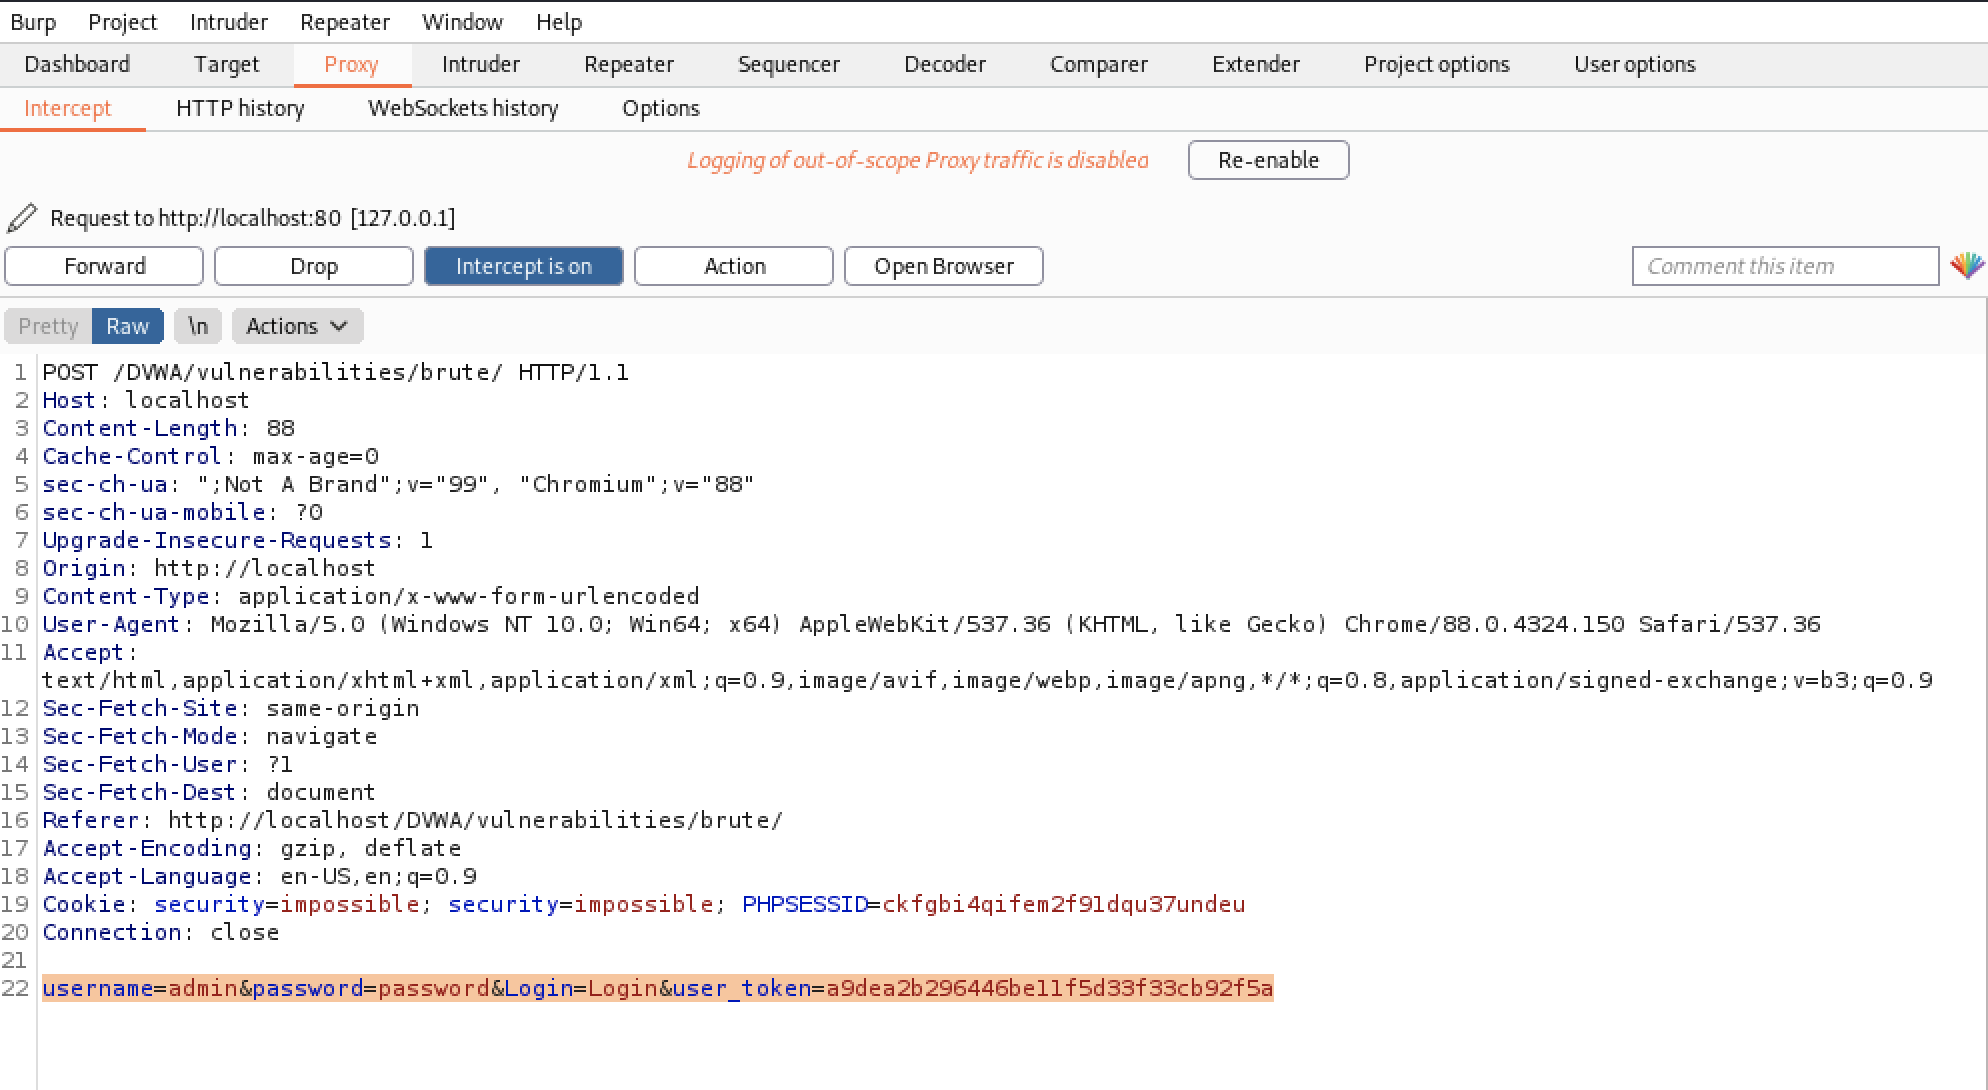
\includegraphics[scale=0.4]{2}
\caption{Interception de requête d'authentification comportant un session ID}
\end{figure}

En supposant que le nom d’utilisateur est “admin”, nous utilisons Hydra en ajoutant les informations obtenues dans Burp précédemment afin de d'attaquer par bruteforce le mot de passe de l'utilisateur. Malheureusement, Hydra semble ne pas fonctionner dans ce cas. On peut voir sur le screen ci-dessous que le mot de passe “password” est  essayé mais sans succès.
\begin{figure}[H]
\centering
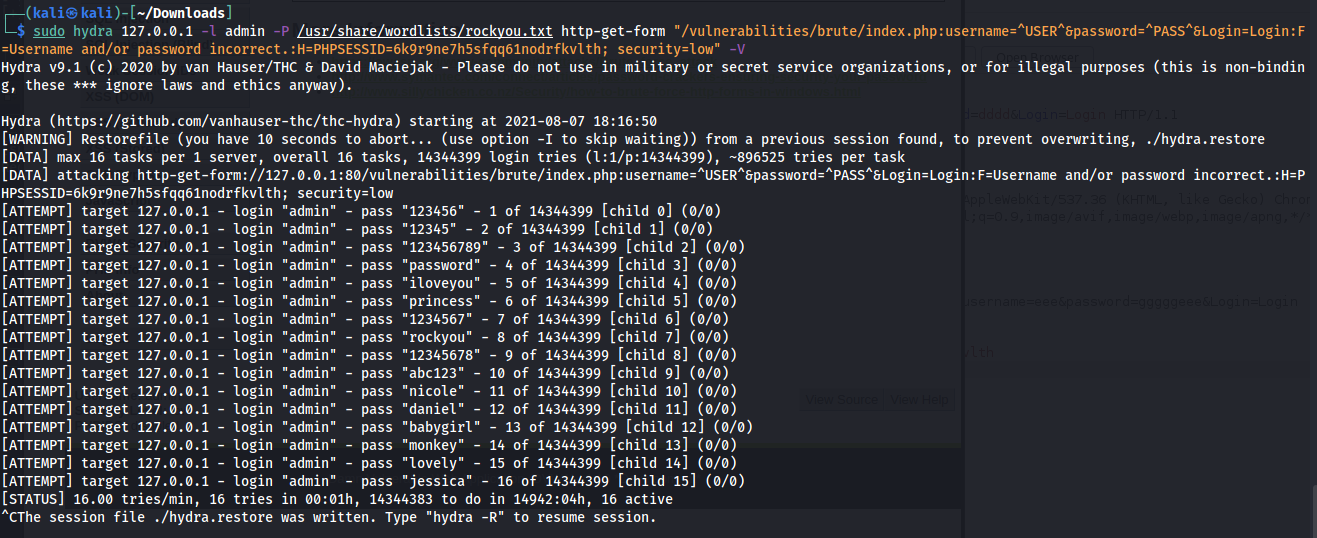
\includegraphics[scale=0.4]{Image9}
\caption{Tentative d'utilisation de Hydra}
\end{figure}
Nous allons alors changer d’outil afin utiliser wfuzz, un logiciel qui sert à faire du fuzzing sur les sites web. Le mot de passe est bien trouvé en 222 requêtes.
\begin{figure}[H]
\centering
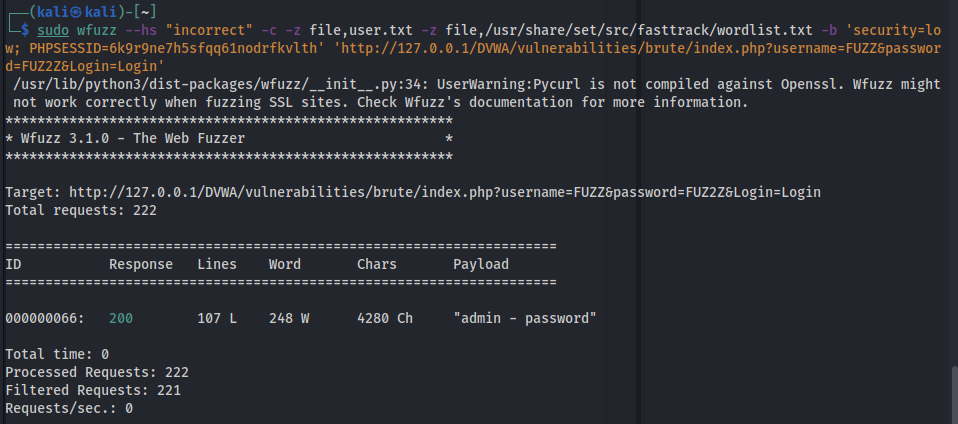
\includegraphics[scale=0.4]{Image10}
\caption{Attaque avec wfuzz}
\end{figure}
Nous créons un dictionnaire de mots de passe à l’aide de l’outil elpscrk pour les utilisateurs admin, pablo et smithy. Cependant, comme ce sont des personnages fictifs, nous ajoutons de fausses données dans les champs d’informations.
\begin{figure}[H]
\centering
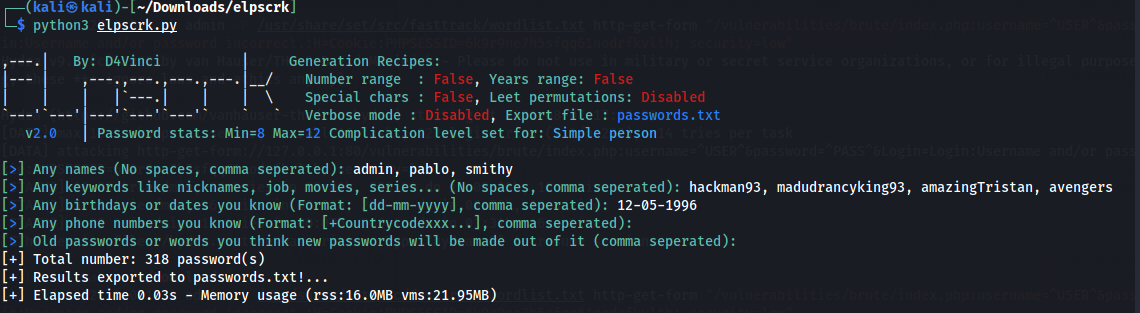
\includegraphics[scale=0.4]{Image11}
\caption{Utilisation de elpscrk}
\end{figure}
\begin{figure}[H]
\centering
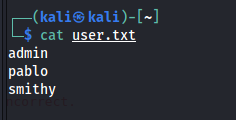
\includegraphics[scale=0.4]{Image12}
\caption{Utilisateur}
\end{figure}
\begin{figure}[H]
\centering
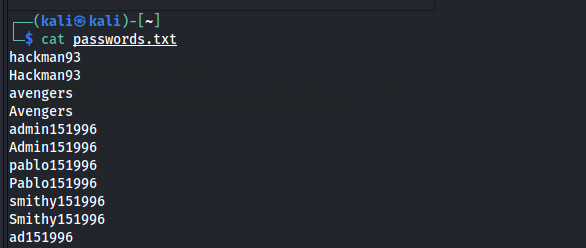
\includegraphics[scale=0.4]{Image13}
\caption{Mots de passe générés par elpscrk}
\end{figure}
Nous lançons le brute force avec ces deux dictionnaires mais ayant mit des informations fictives le brute force ne peut pas aboutir.
\begin{figure}[H]
\centering
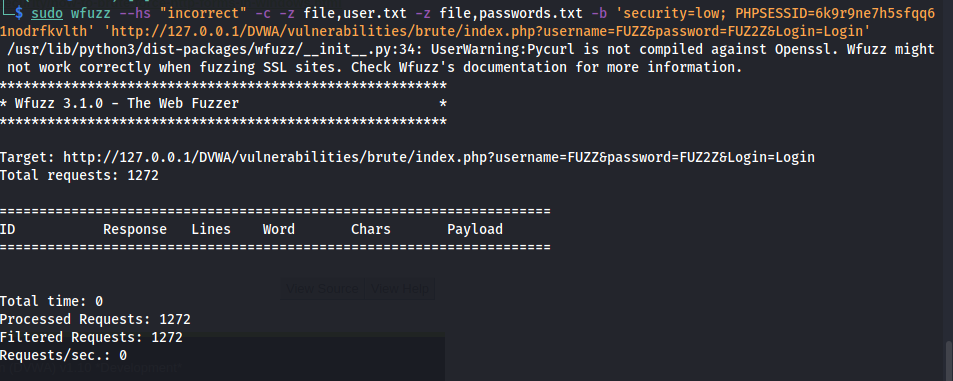
\includegraphics[scale=0.4]{Image14}
\end{figure}

\section{Blind SQL Injection}

Lors de l'envoi du formulaire, on constate que le champ renseigné dans l'input est passé dans la requête en tant qu'un paramètre GET, envoyé au serveur. Nous allons donc essayer plus tard de jouer avec ce paramètre.

\begin{figure}[H]
\centering
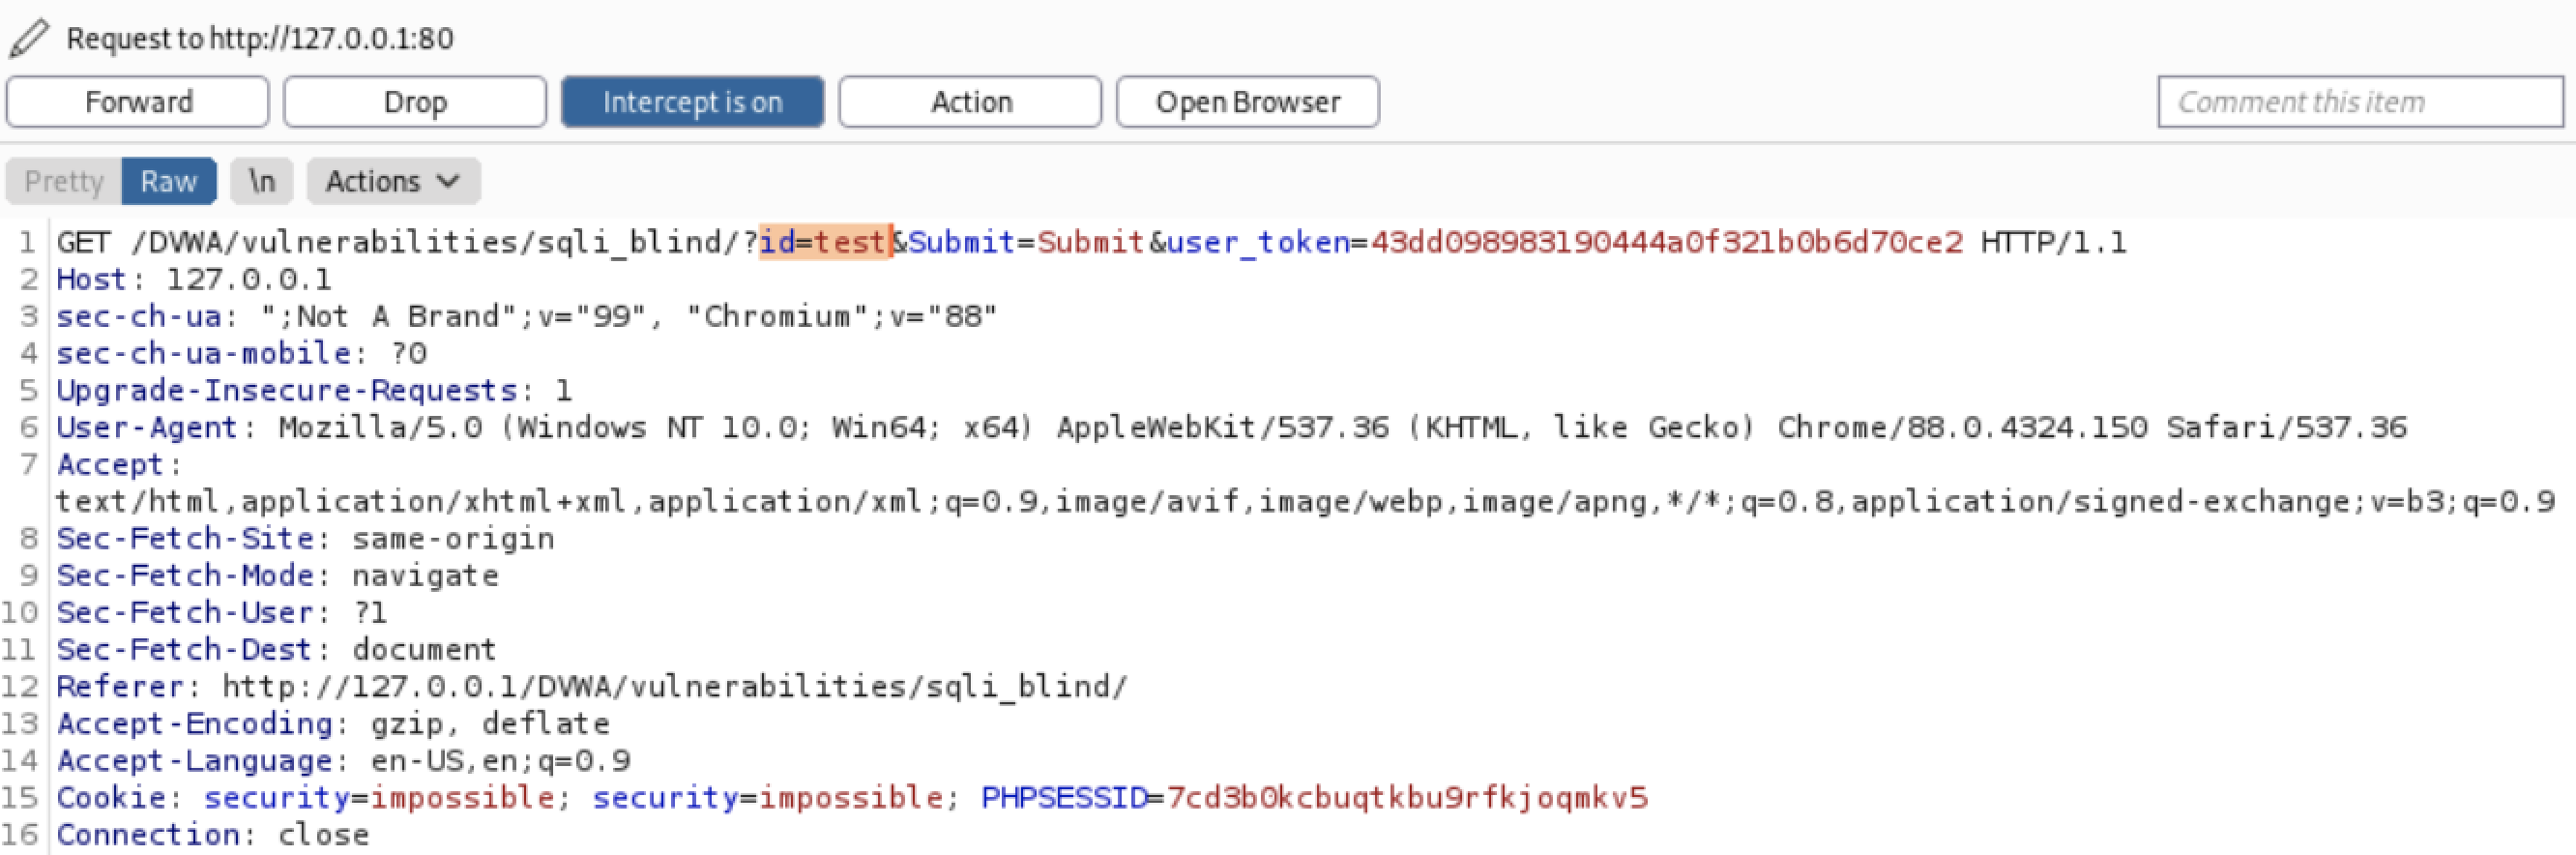
\includegraphics[scale=0.4]{3}
\caption{Format de la requête GET à exploiter}
\end{figure}

Afin d'obtenir beaucoup plus d'informations sur de potentielles failles SQL présentes sur la page, nous utilisons sqlmap. 
sqlmap est un outil qui automatise le processus de détection et d'exploitation des failles d'injection SQL. D'autres outils peuvent être utilisés comme bbqsql mais sqlmap est très bien adapté à notre cas.

La première commande nous conseille deux payloads qui peuvent potentiellement exploite rune faille SQL mais n'ont pas été un succès.
Cependant, il a été possible d'énumérer les tables existantes sur la base de données MySQL utilisée par le serveur du site grâce à l'option -D dvwa –tables. Une fois les tables énumérées, nous savons que nous avons à présent accès au contenu de la base de données! 

\begin{figure}[H]
\centering
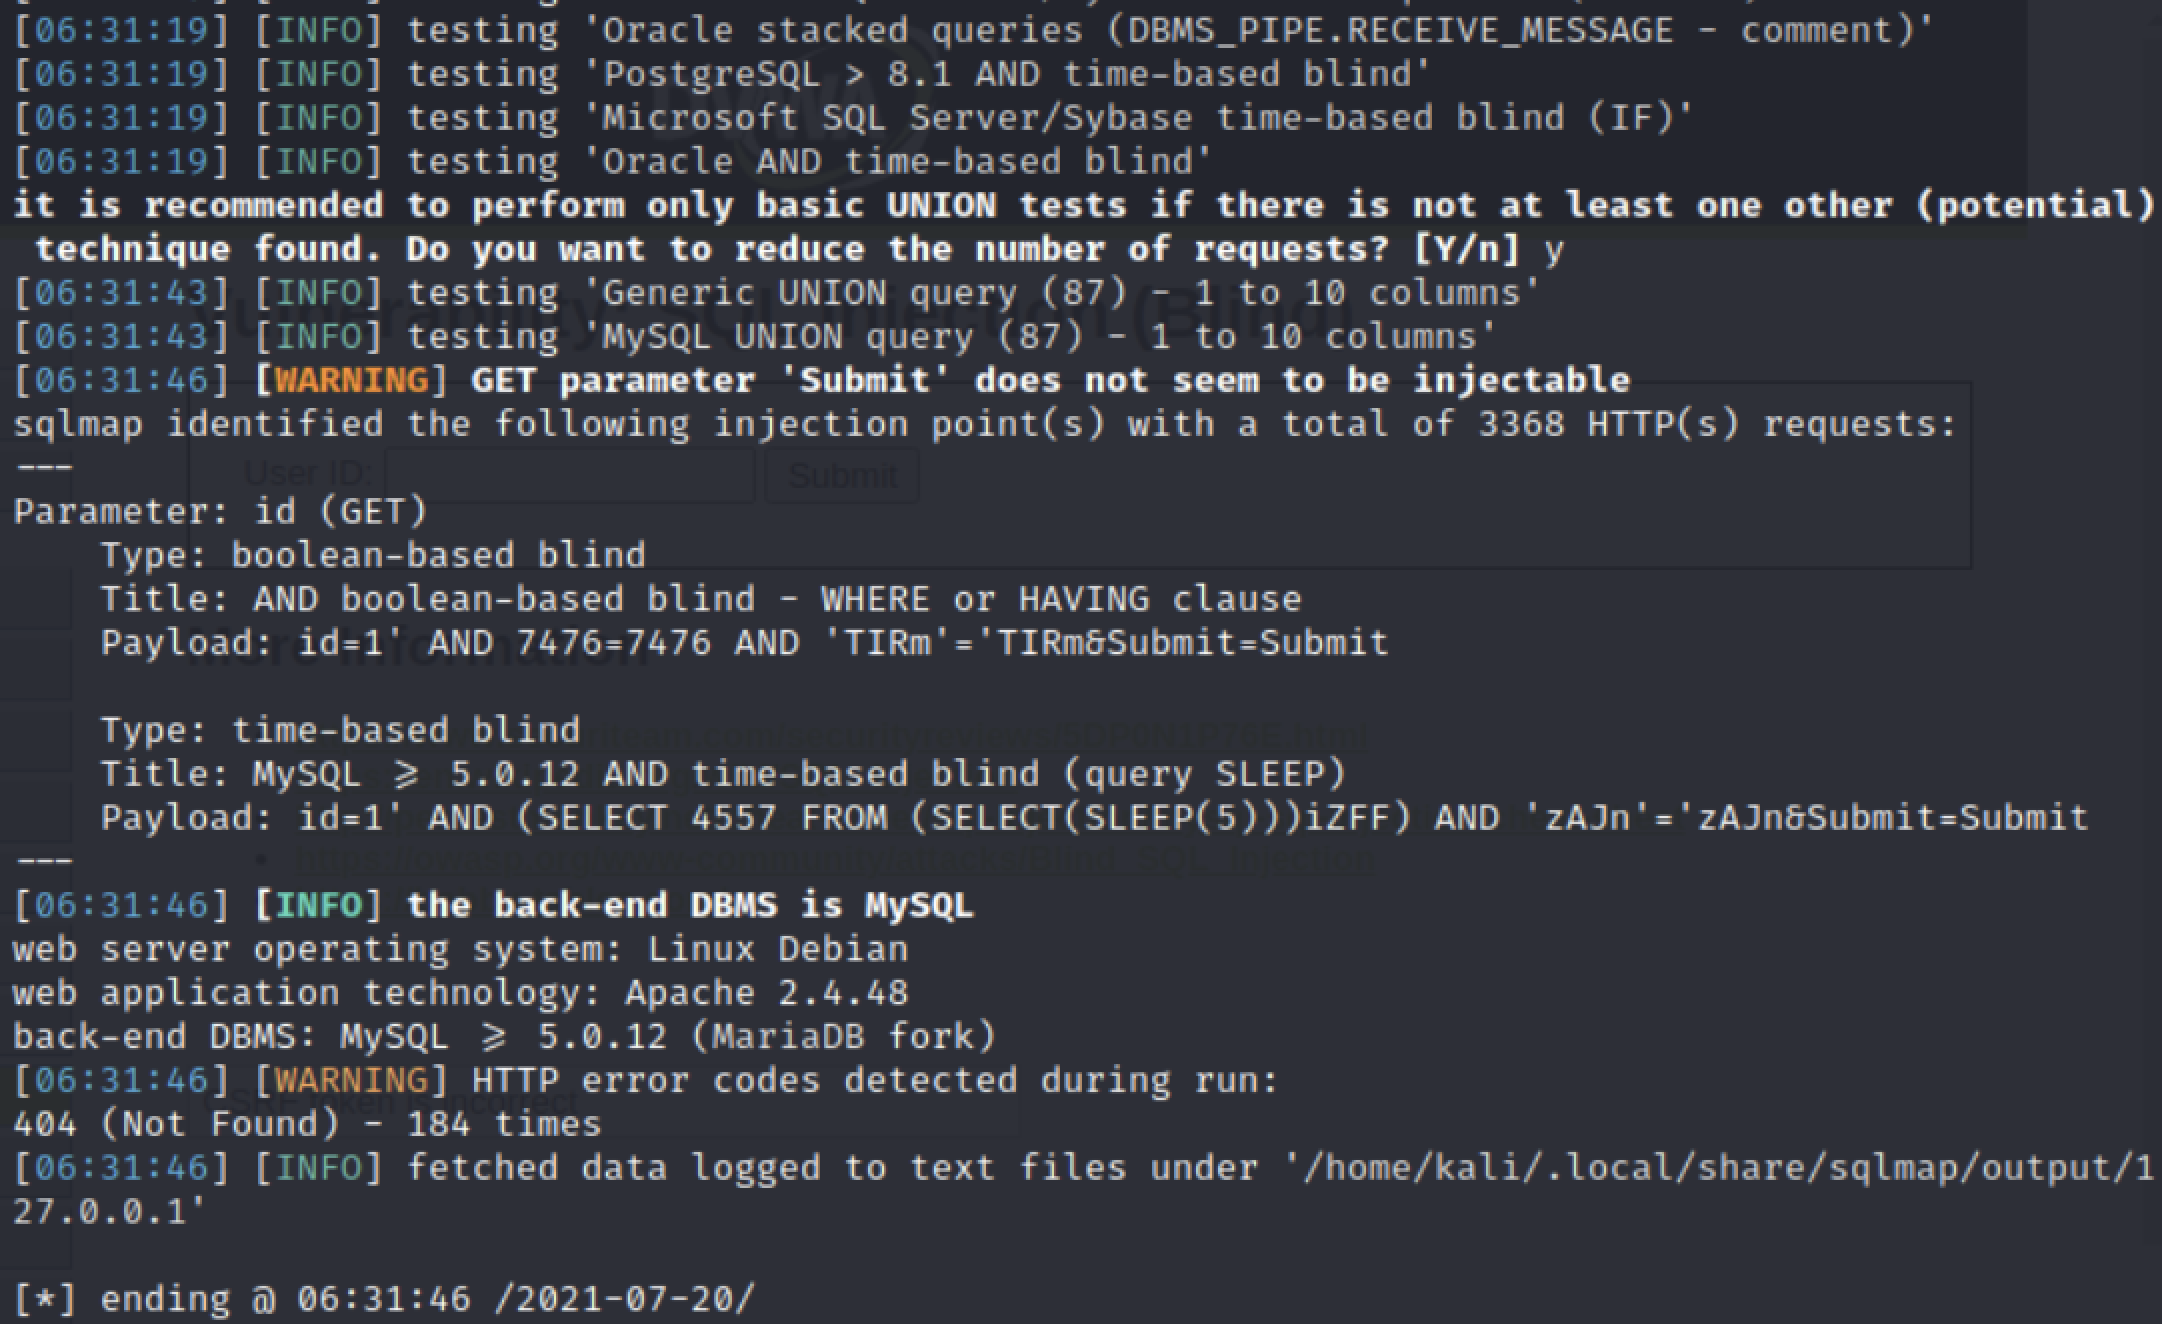
\includegraphics[scale=0.4]{4}
\caption{Listing des tables présentes dans la base de données}
\end{figure}

La base de données contient deux tables: guestbook et users. Dans un premier temps, analysons le contenu de la table users puisqu'on se doute qu'elle contient des informations qui pourraient nous intéresser. L'option -T users -columns nous permet d'afficher le schéma de la table users.

\begin{figure}[H]
\centering
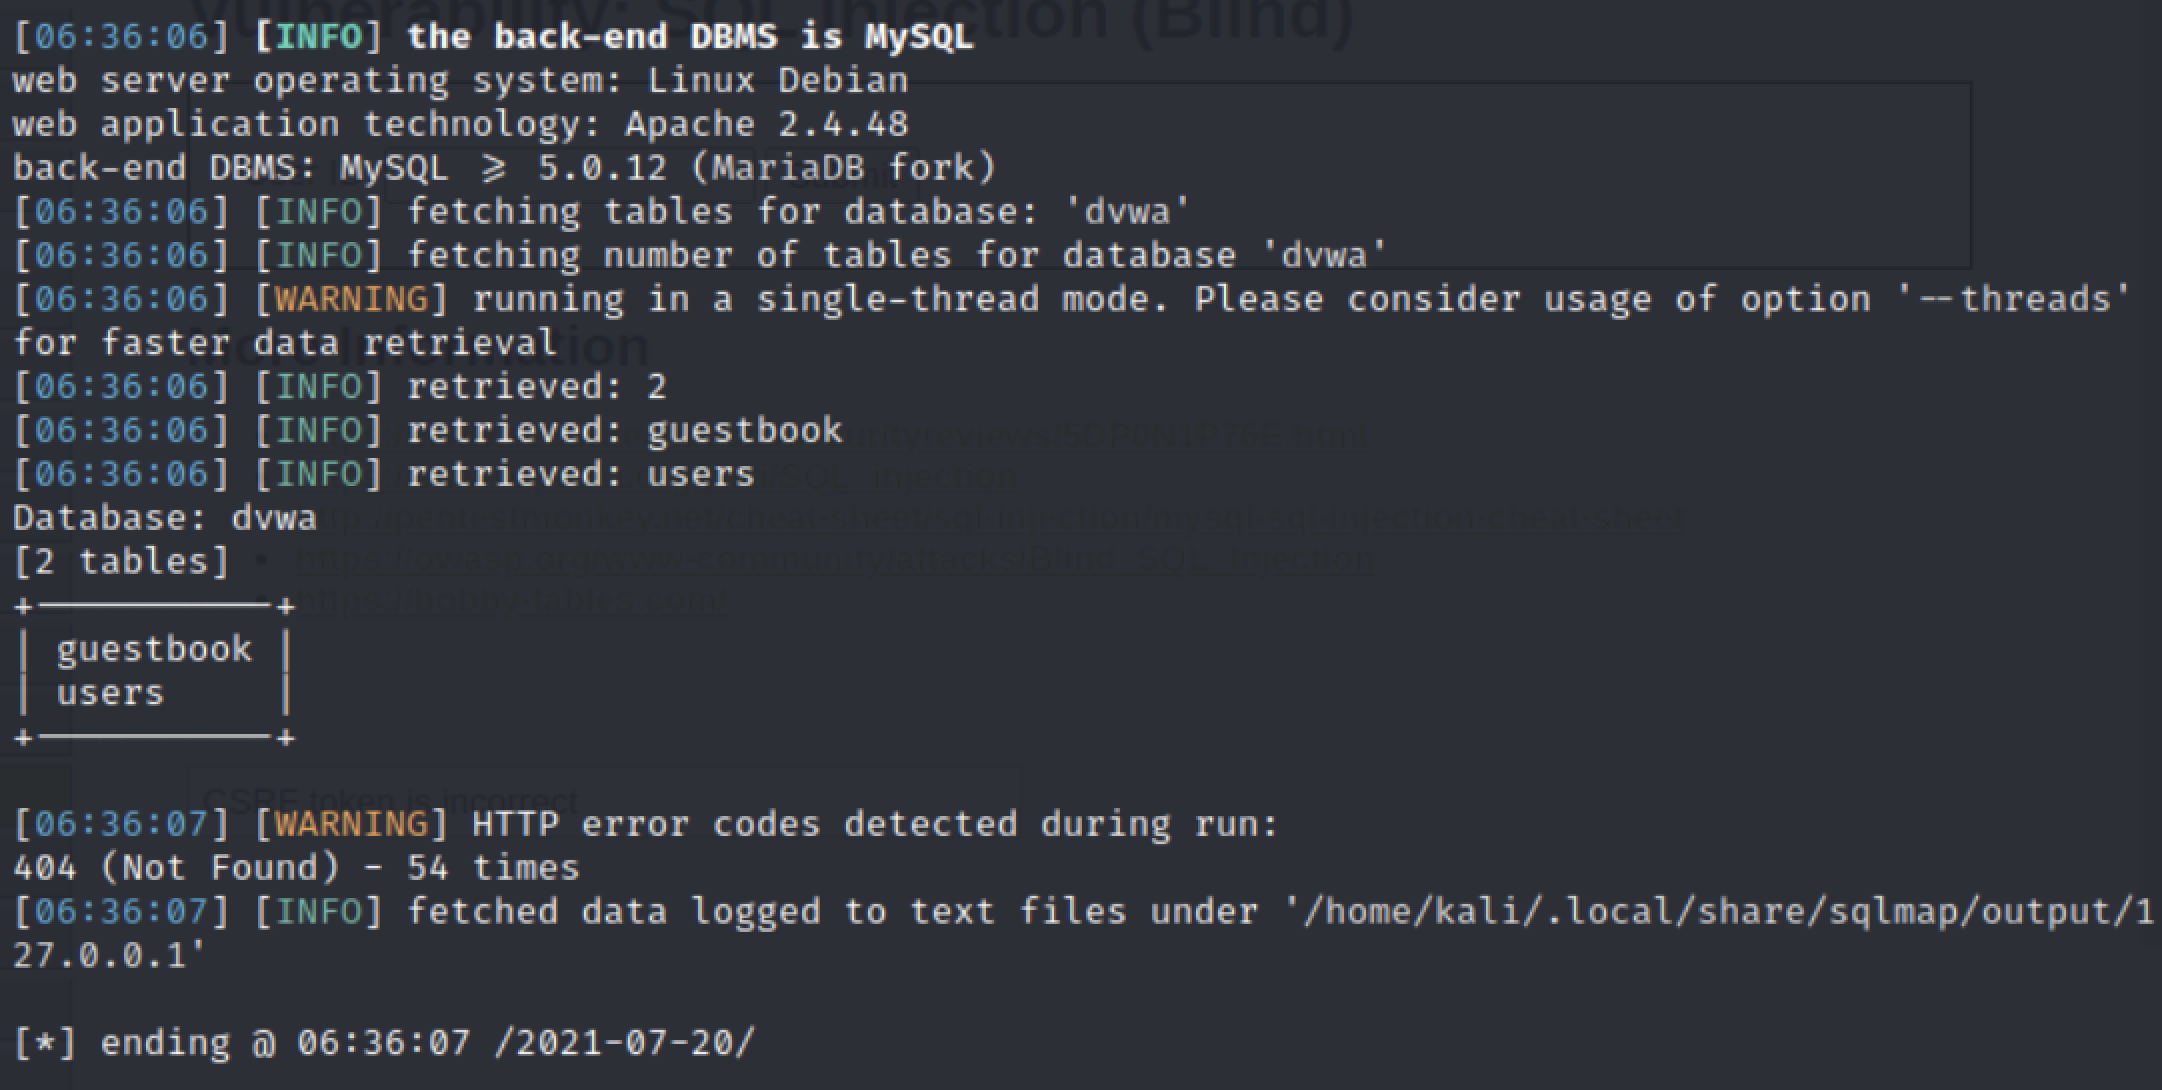
\includegraphics[scale=0.4]{5}
\caption{Schéma de la table users}
\end{figure}

Nous voyons des champs très intéressants comme user ou password. Essayons maintenant de les dumper avec l'option --dump.

\begin{figure}[H]
\centering
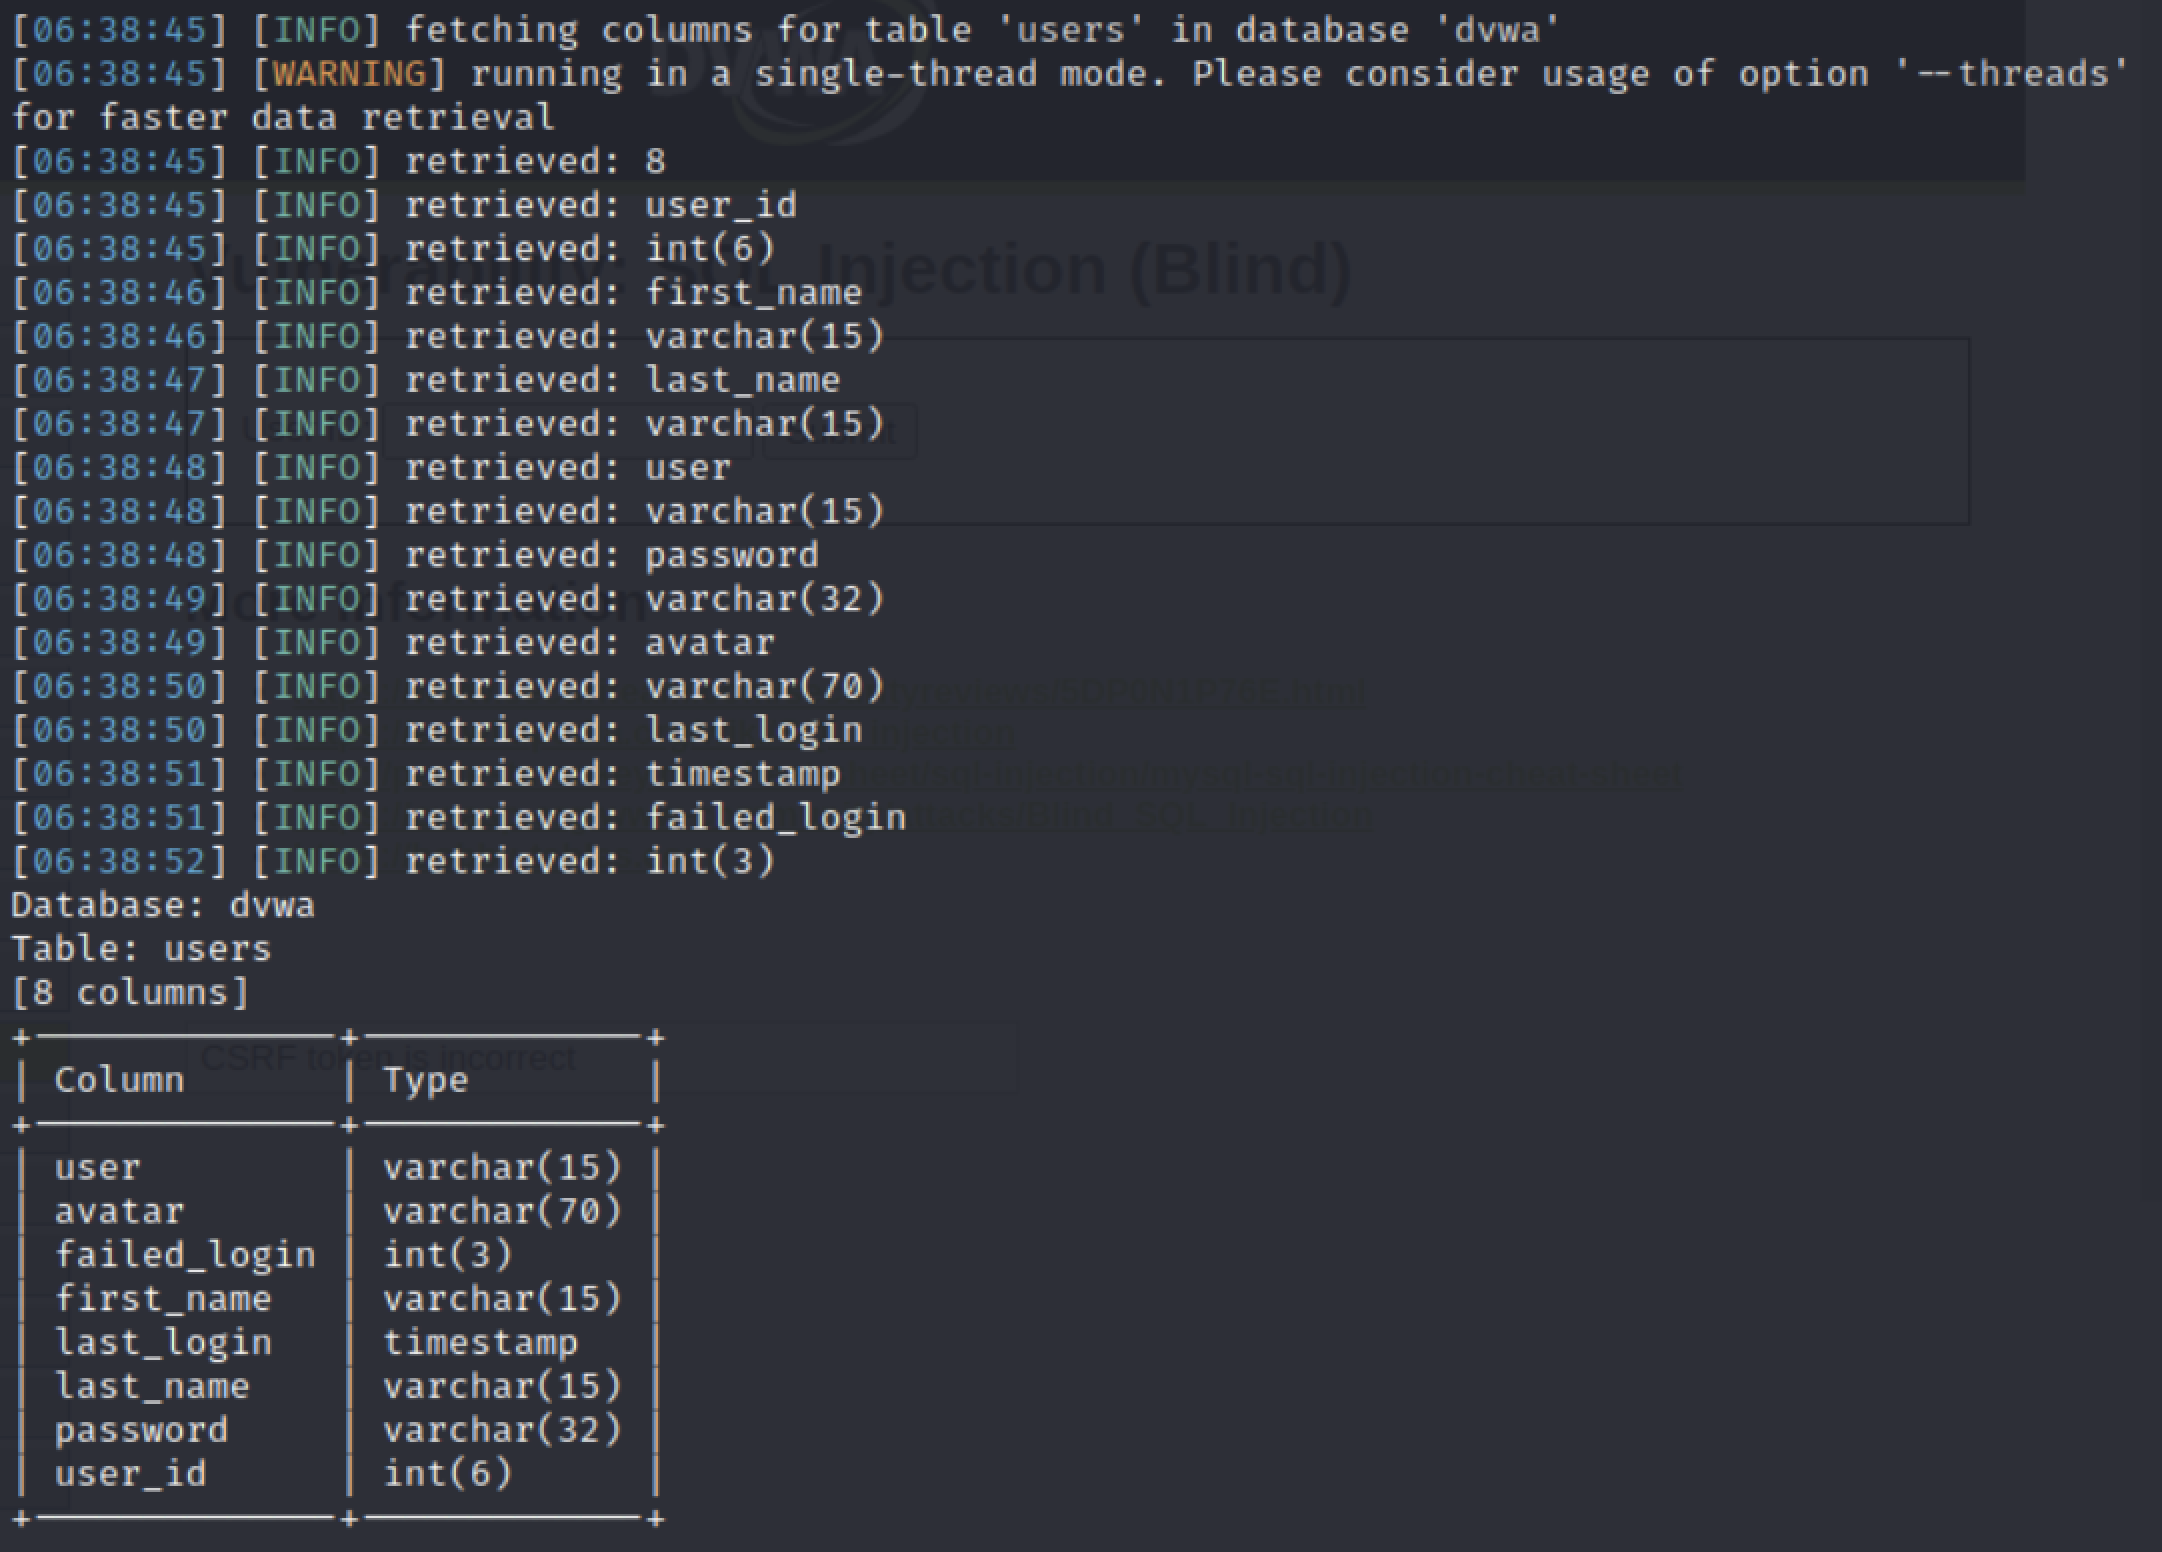
\includegraphics[scale=0.4]{6}
\caption{Dump du contenu de la table users}
\end{figure}

Nous obtenons la liste complète des utilisateurs inscrits sur le site. Les mots de passe sont hashés en MD5, mais l'outil sqlmap propose une méthode permettant d'effectuer une attaque par dictionnaire et rainbow tables dessus afin d'essayer de retrouver les mots de passe en clair.

\begin{figure}[H]
\centering
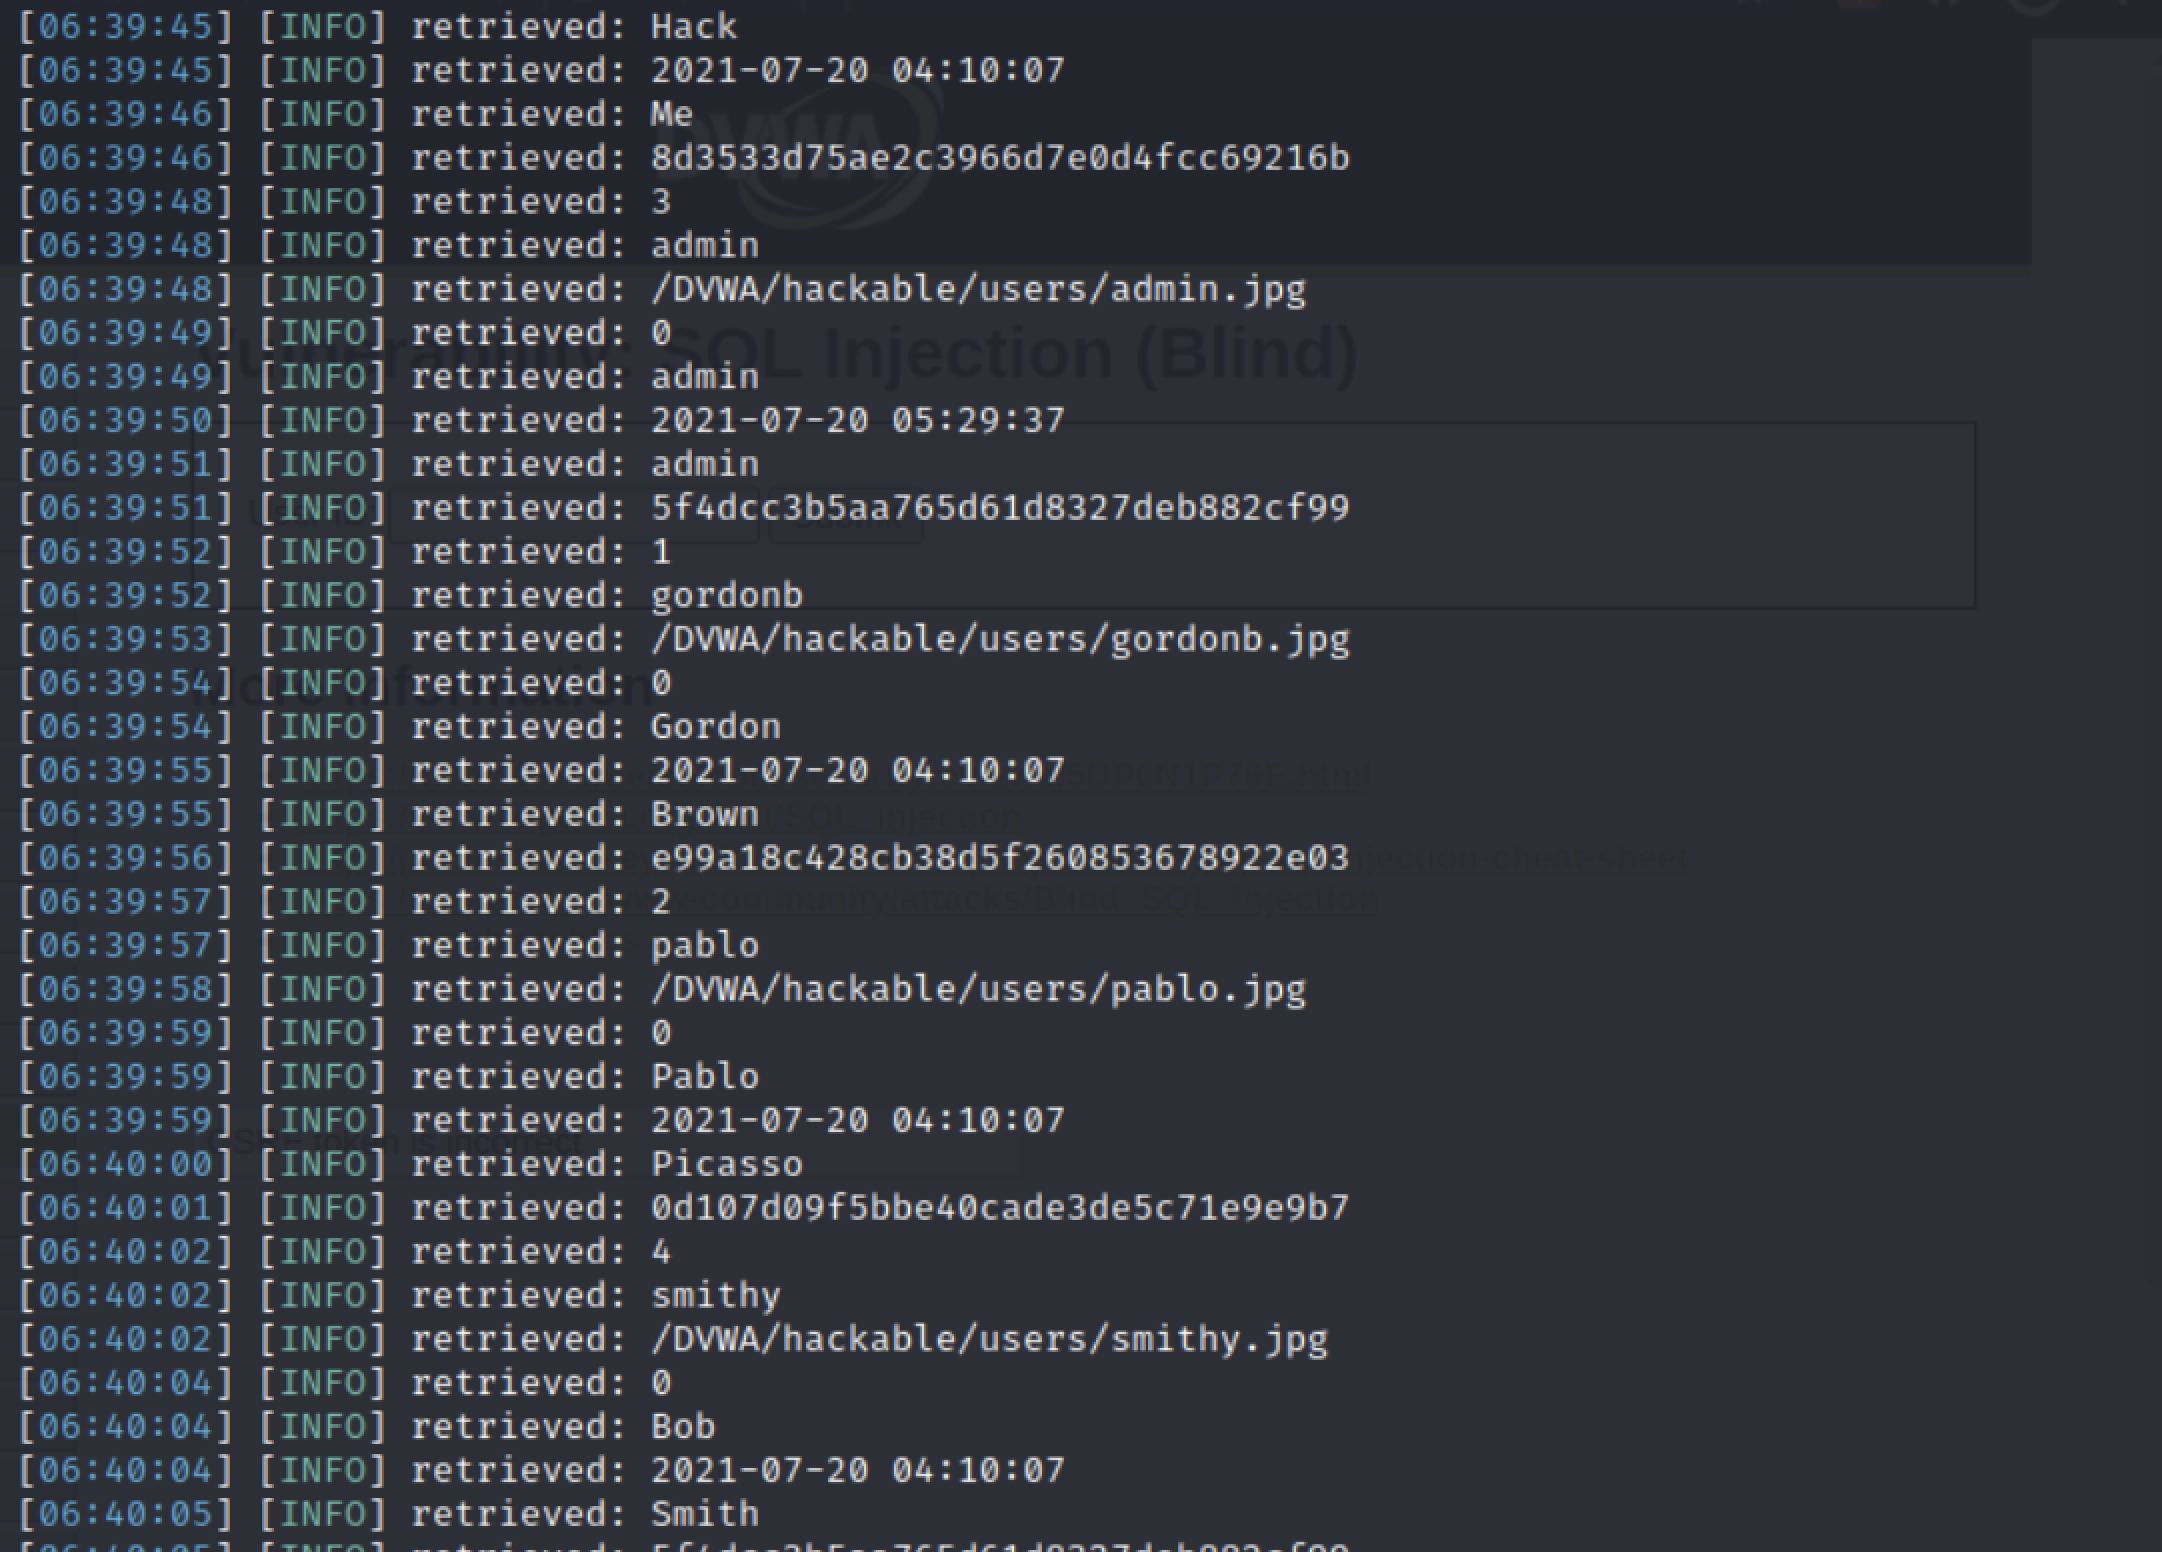
\includegraphics[scale=0.4]{7}
\caption{Dump du contenu de la table users}
\end{figure}

\begin{figure}[H]
\centering
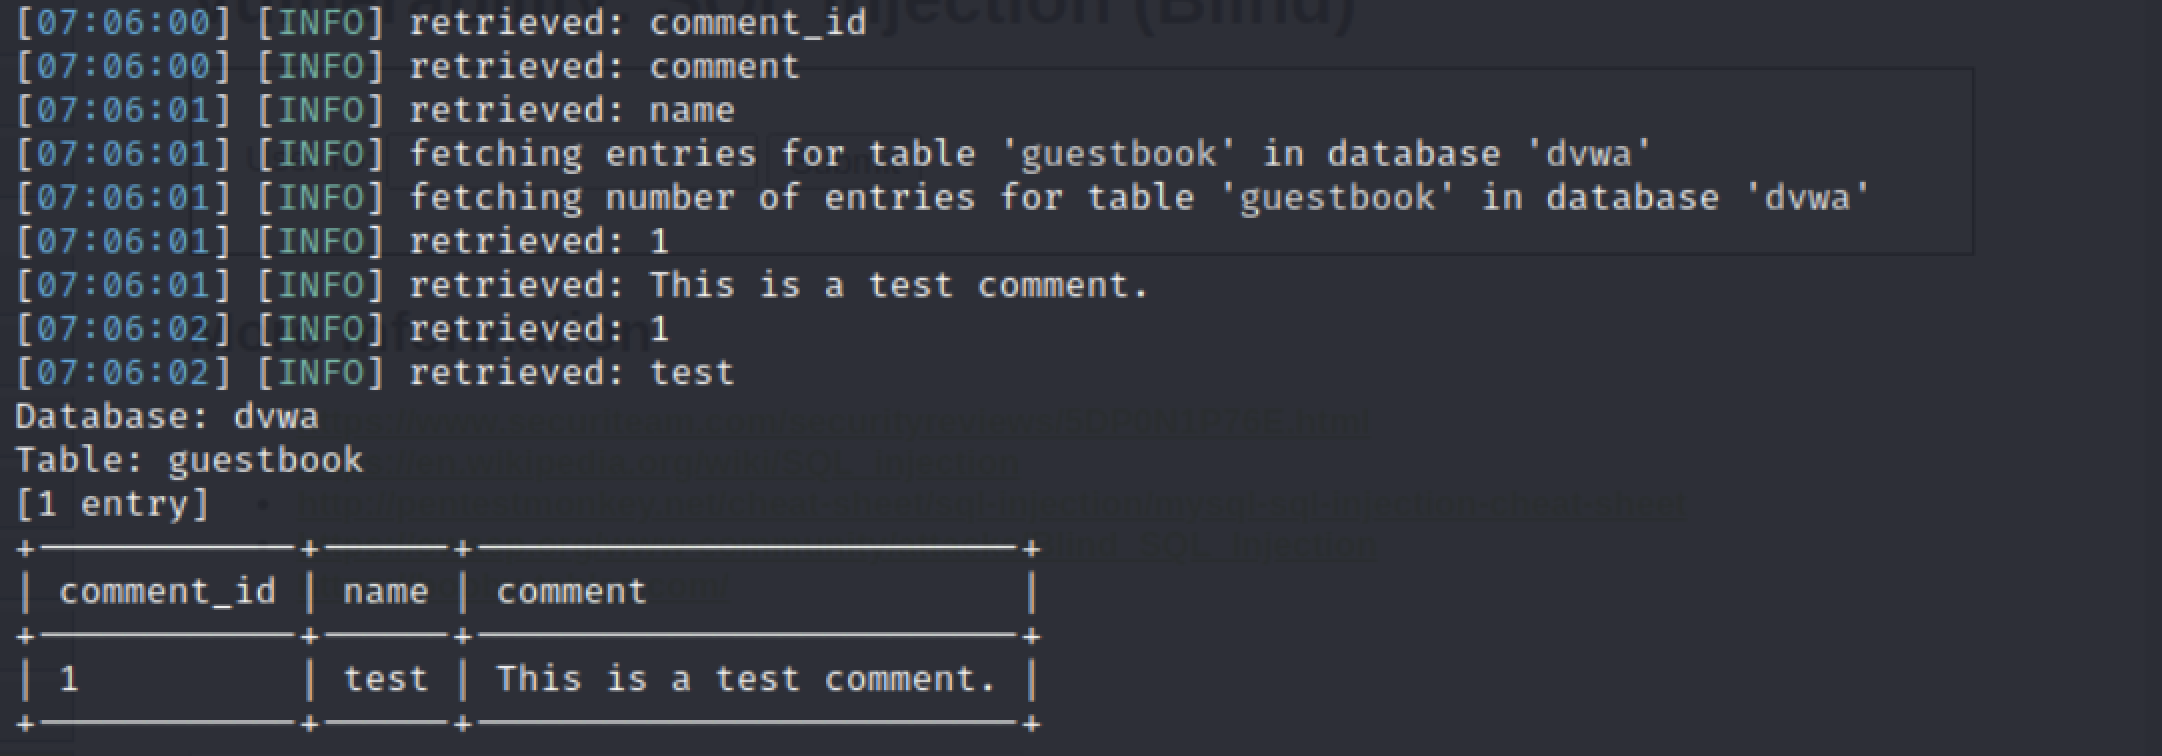
\includegraphics[scale=0.4]{9}
\caption{Dump du contenu de la table guestbook}
\end{figure}

Cinq mots de passe sont obtenus en quelques secondes, nous allons pouvoir les utiliser pour nous connecter au site en tant que ces utilisateurs. La table guestbook quant à elle ne contient qu'un commentaire.

\begin{figure}[H]
\centering
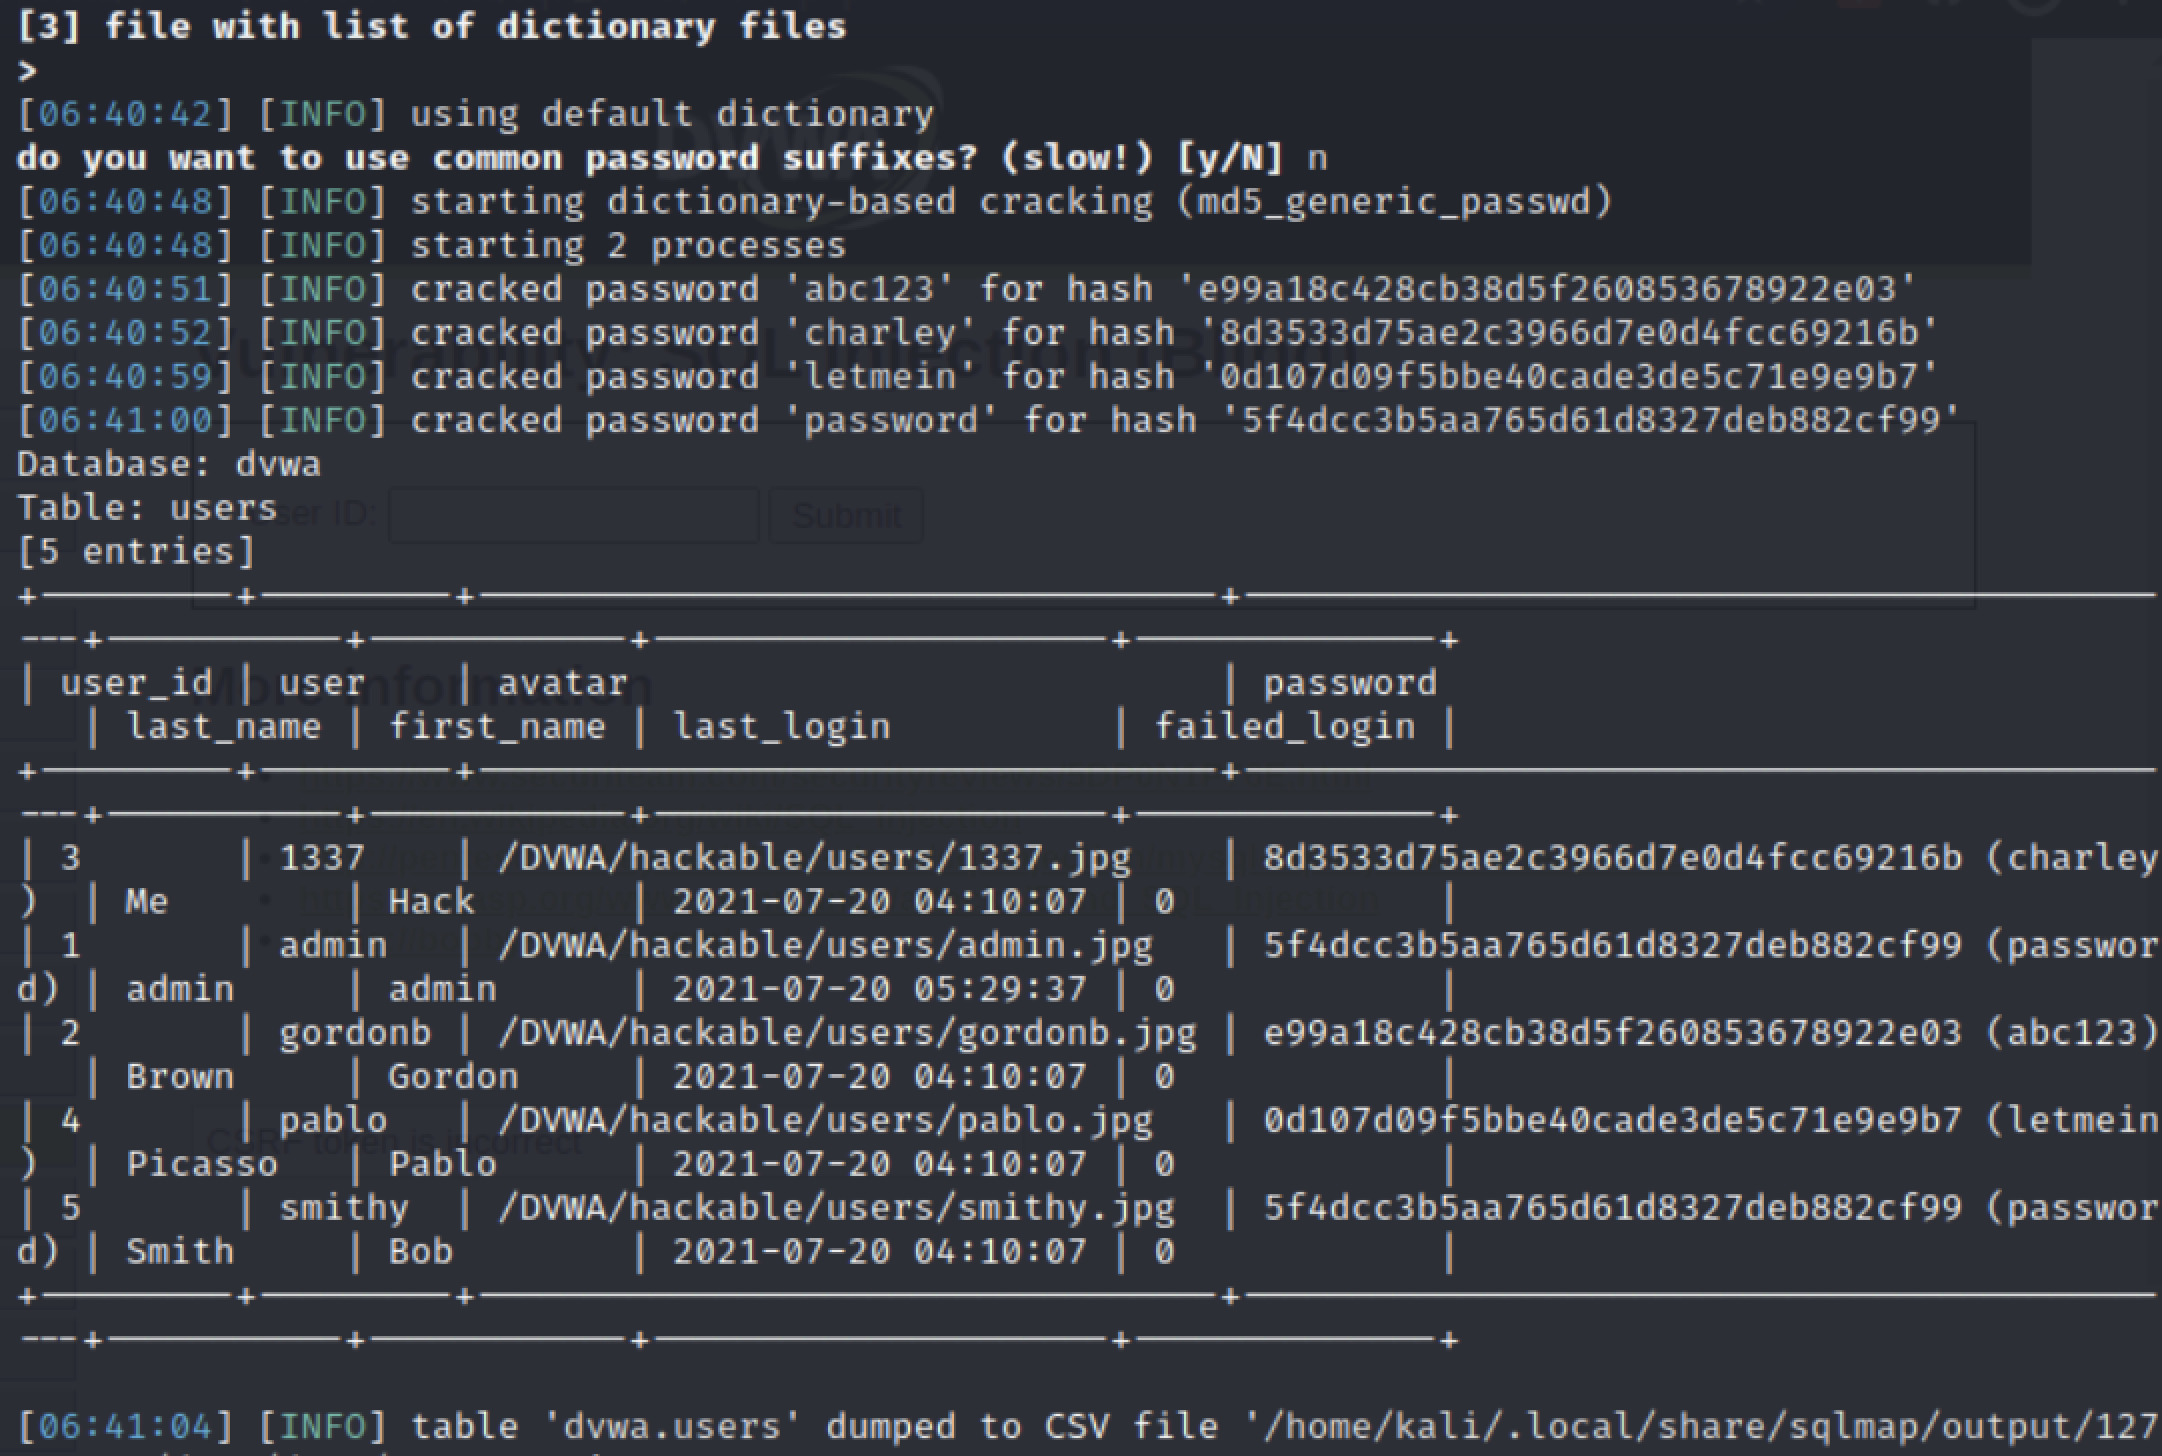
\includegraphics[scale=0.4]{8}
\caption{Découverte des mots de passe par comparaison de hashs}
\end{figure}

Enfin, il est possible de récupérer les photos de profil utilisateur etc.

\begin{figure}[H]
\centering
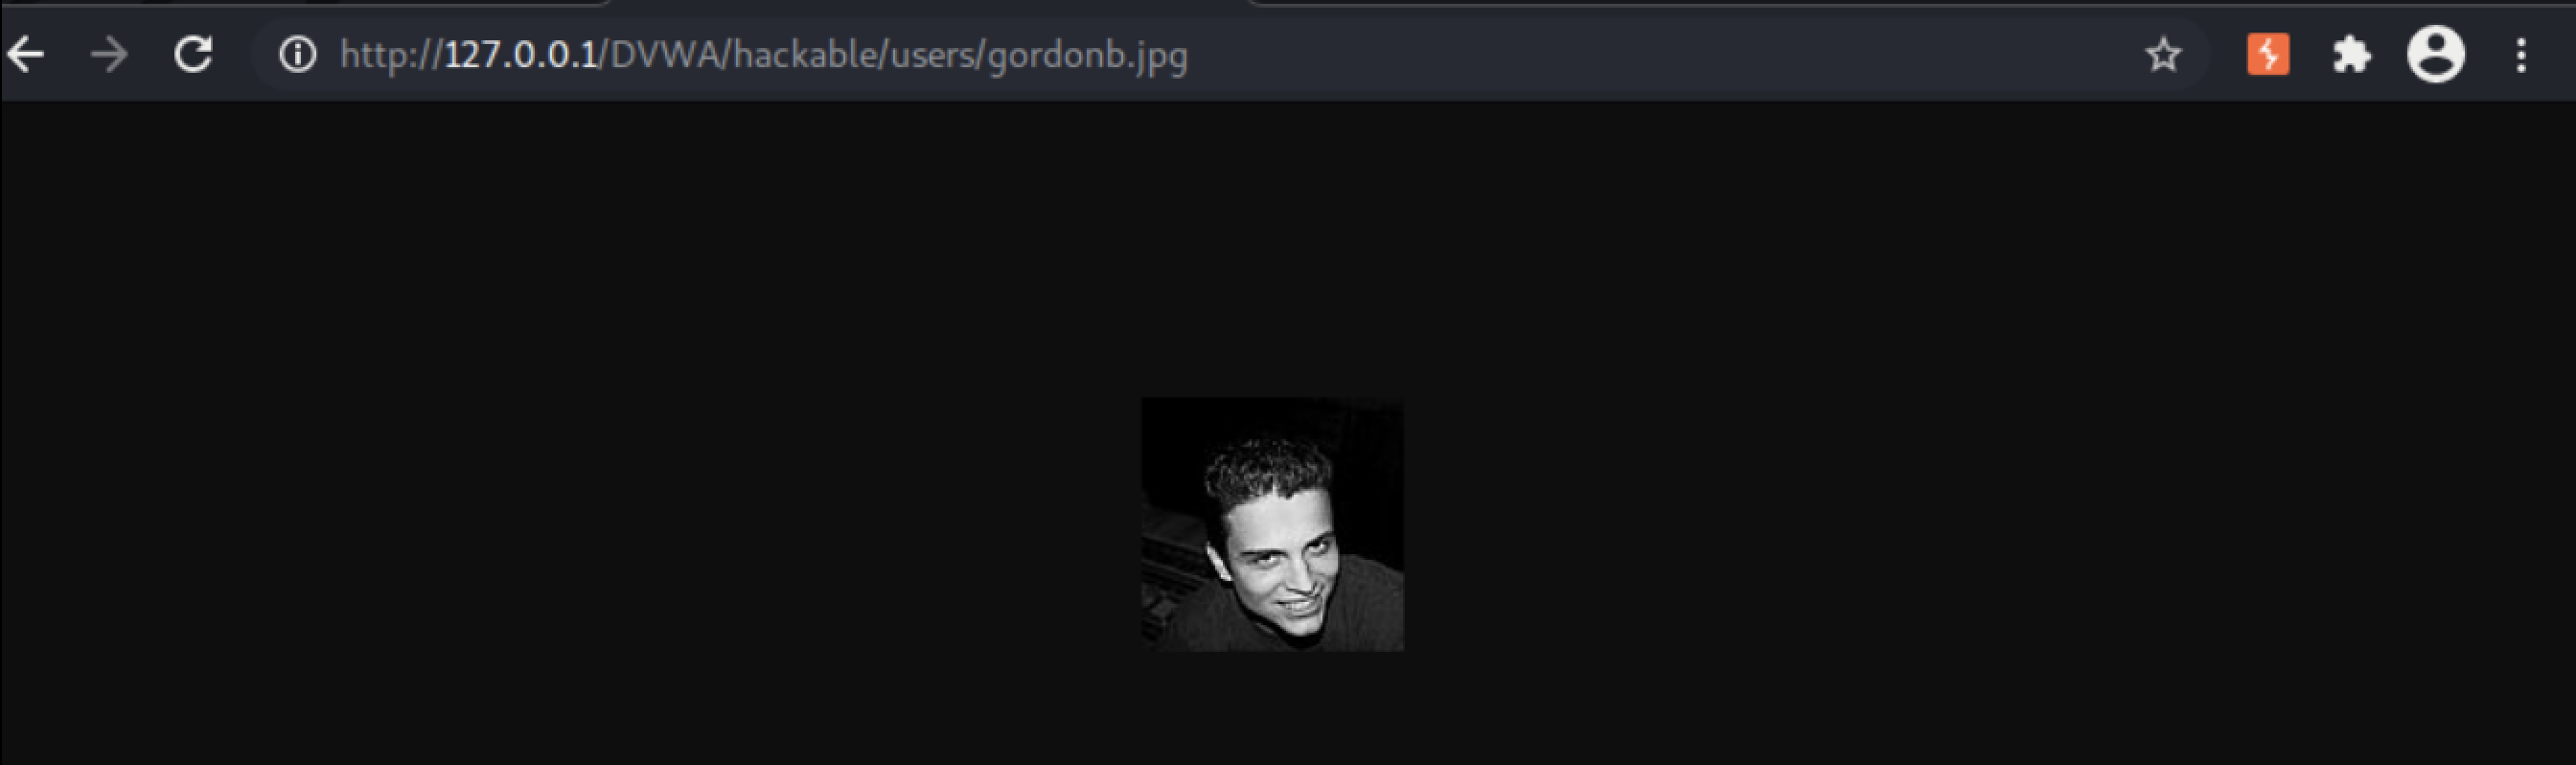
\includegraphics[scale=0.4]{10}
\caption{Photo de profil de l'utilisateur Gordon B.}
\end{figure}

\section{Stored XSS}
Les attaques XSS se produisent lorsqu'un attaquant utilise une application Web pour envoyer du code malveillant, généralement sous la forme d'un script côté navigateur, à un autre utilisateur final. Sur les trois types de XSS, les attaquants sont les plus intéressés par les stored XSS . La raison en est que la portée du code malveillant est énorme. Il faut moins de ressources pour cibler un plus grand nombre de victimes. Et une fois le code malveillant en place, son effet est continu. Si la stored XSS n'est pas identifiée et atténuée, le code malveillant continuera à faire son travail pour de nombreux utilisateurs et peut durer pendant des années.

\begin{figure}[H]
\centering
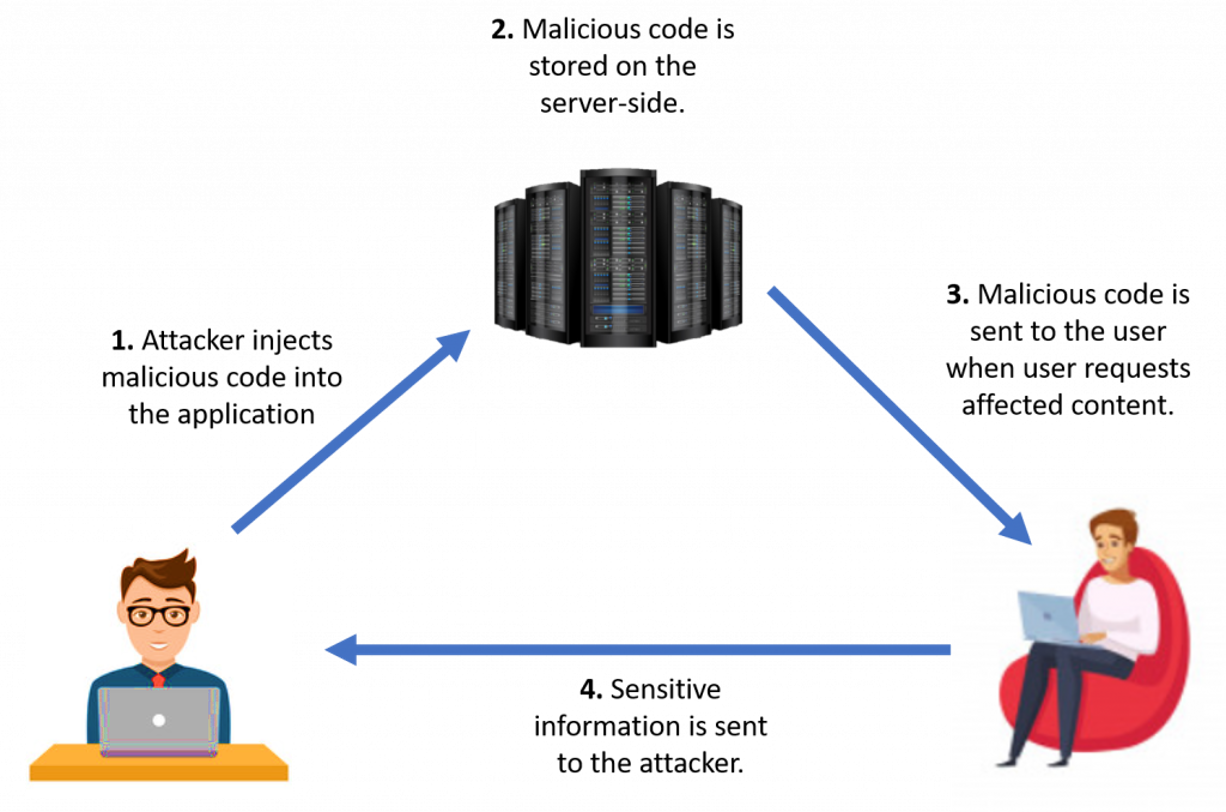
\includegraphics[scale=0.4]{11}
\caption{Stored XSS}
\end{figure}

\subsection{Low}
Ce cas est celui le plus trivial, une faille XSS est directement exploitable, sans parsing ni échappement de caractère côté serveur. Il est alors possible d'injecter du html, css et javascript à travers l'input.

Etant donné que le contenu que nous avons injecté est stocké côté serveur (certainement dans une base de données), ce code va revenir à chaque fois que l'utilisateur ira sur cette page, ce qui en fait une attaque qui peut être très très compliquée à détecter et à résoudre.

\begin{figure}[H]
\centering
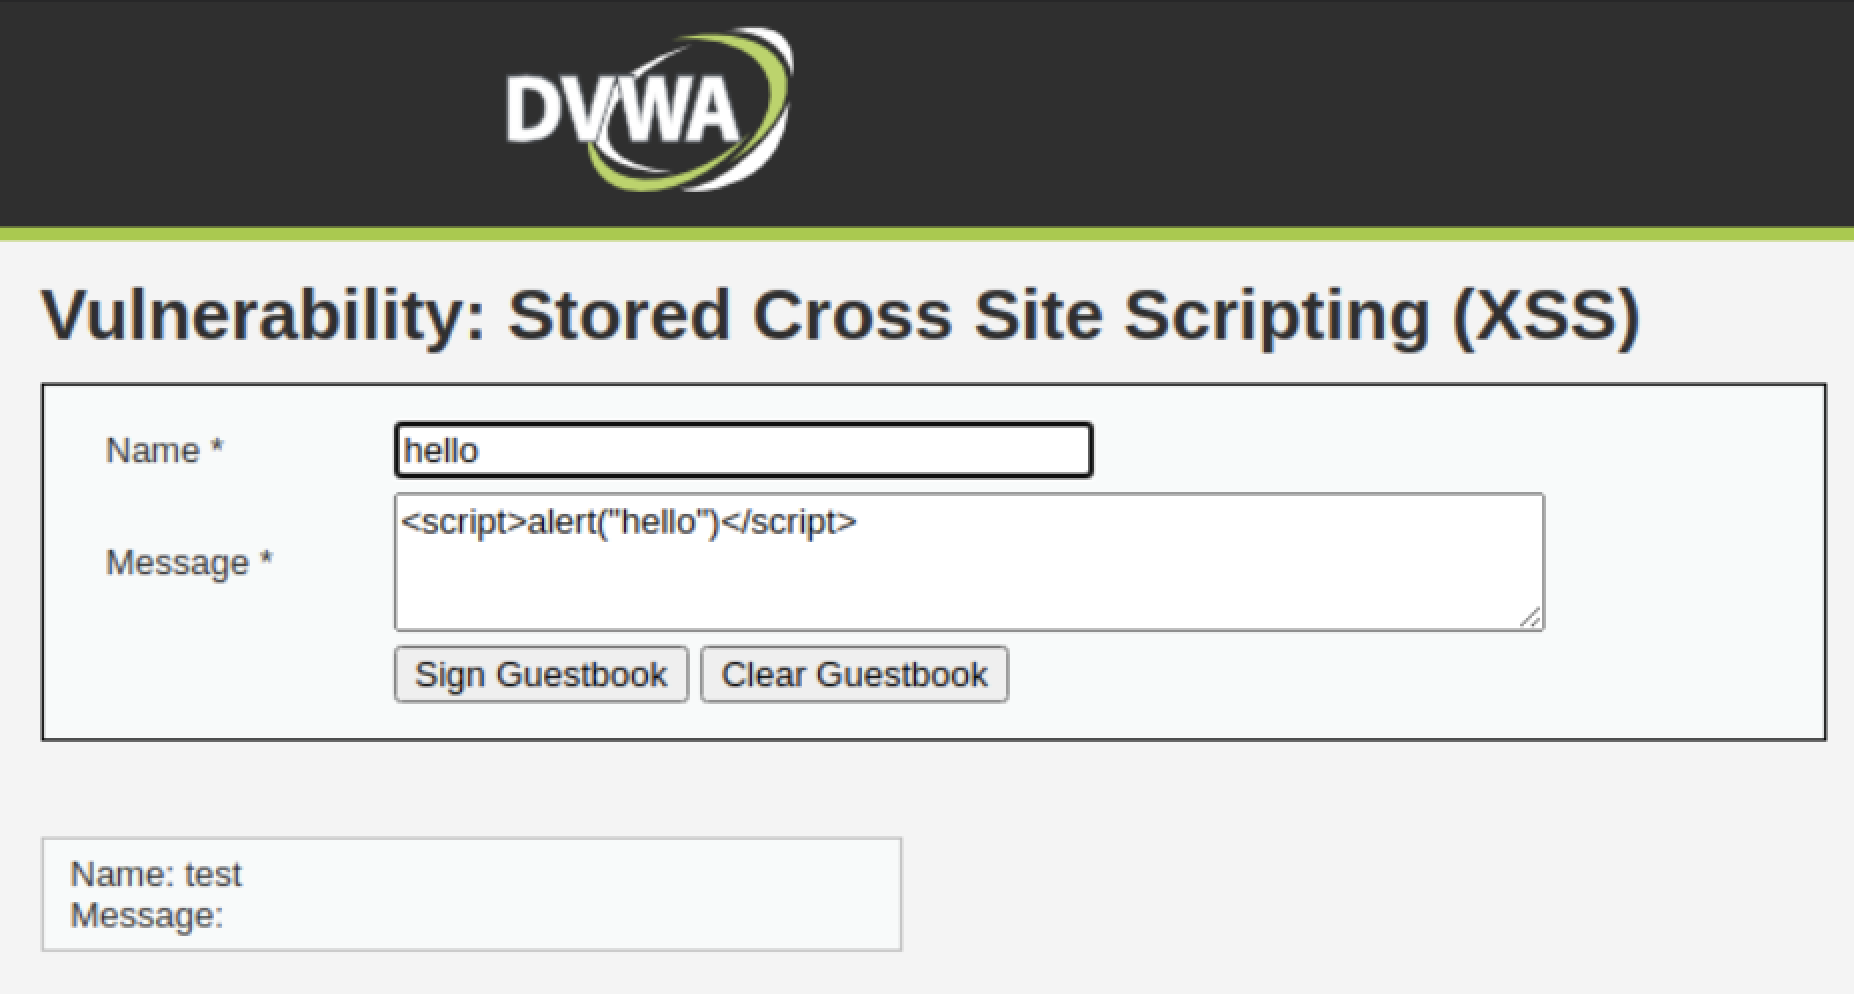
\includegraphics[scale=0.4]{12}
\caption{Exploitation de la faille}
\end{figure}

Etant donné que du code Javascript peut être exécuté, il est alors possible de rediriger des gens sur une autre page. Afin d'enlever la limite de 50 caractères dans l'input, il suffit d'examiner l'élément puis de modifier la valeur.
Dans un cas réel, cette limite de caractères serait certainement également vérifiée côté serveur afin que ce type de technique soit inutile.

\begin{figure}[H]
\centering
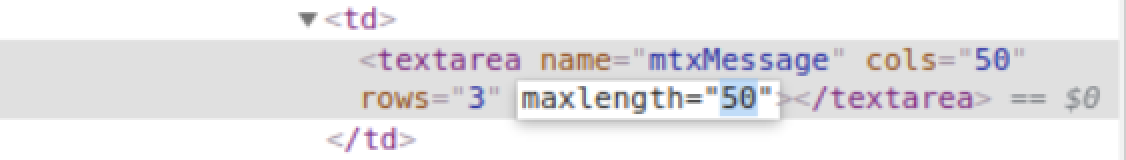
\includegraphics[scale=0.6]{13}
\caption{Augmentation du nombre de caractères écrivables dans l'input}
\end{figure}
\begin{figure}[H]
\centering
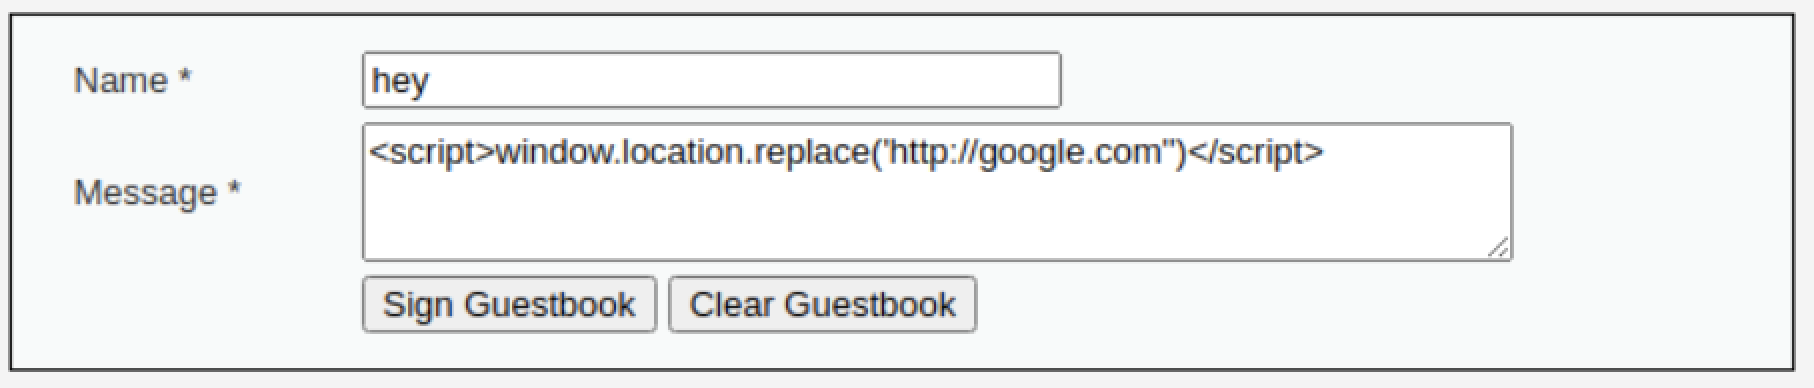
\includegraphics[scale=0.4]{14}
\caption{Redirection vers google.com}
\end{figure}

Il est également possible dans ce cas de voler le cookie de session utilisateur. Etant donné que le code est exécuté côté client, c'est le de cookie de la cible qui sera affiché.

\begin{figure}[H]
\centering
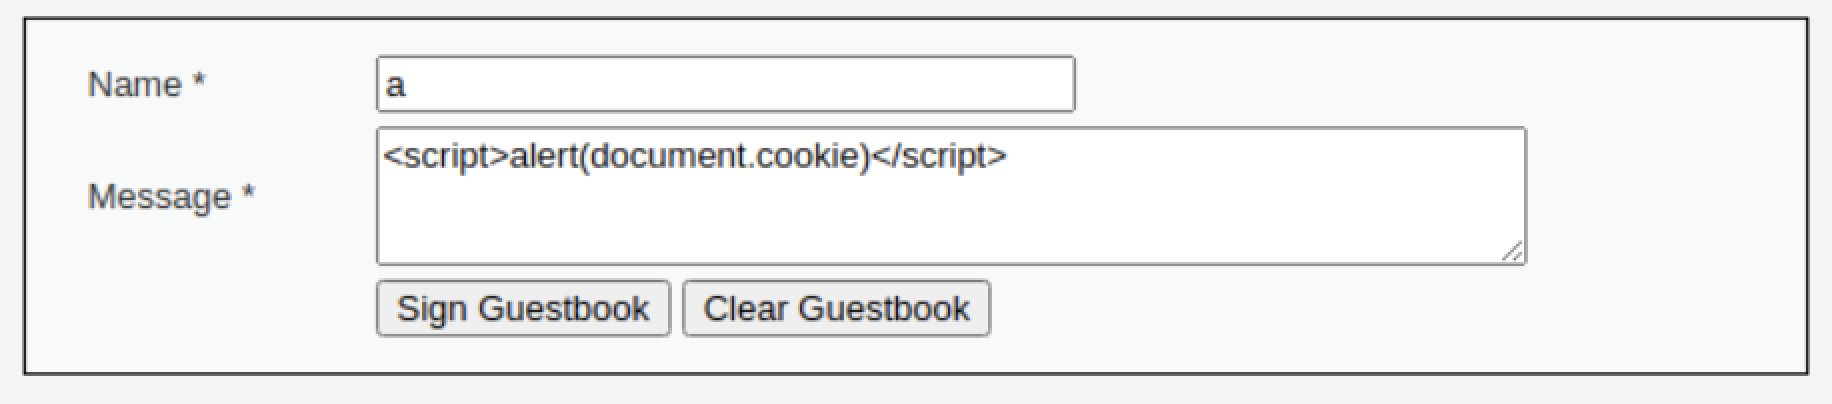
\includegraphics[scale=0.4]{15}
\caption{Affichage de document.cookie}
\end{figure}
\begin{figure}[H]
\centering
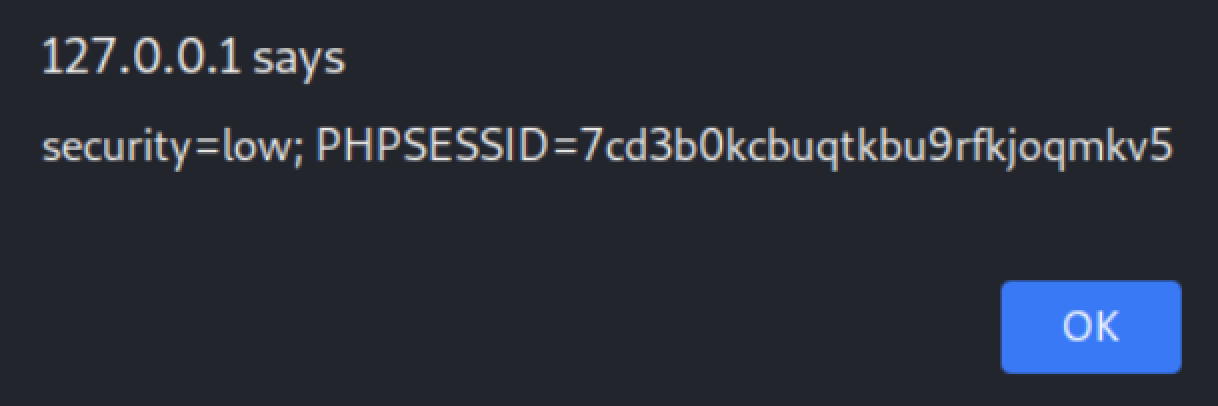
\includegraphics[scale=0.4]{16}
\caption{Résultat}
\end{figure}

\subsection{Medium}
Dans ce cas, la simple injection d'une balise javascript n'a aucun effet puisque les simple quotes sont échappées. Il faut donc trouver une solution 

\section{CSRF}
La page CSRF contient un formulaire permettant le changement du mot de passe.
\begin{figure}[H]
\centering
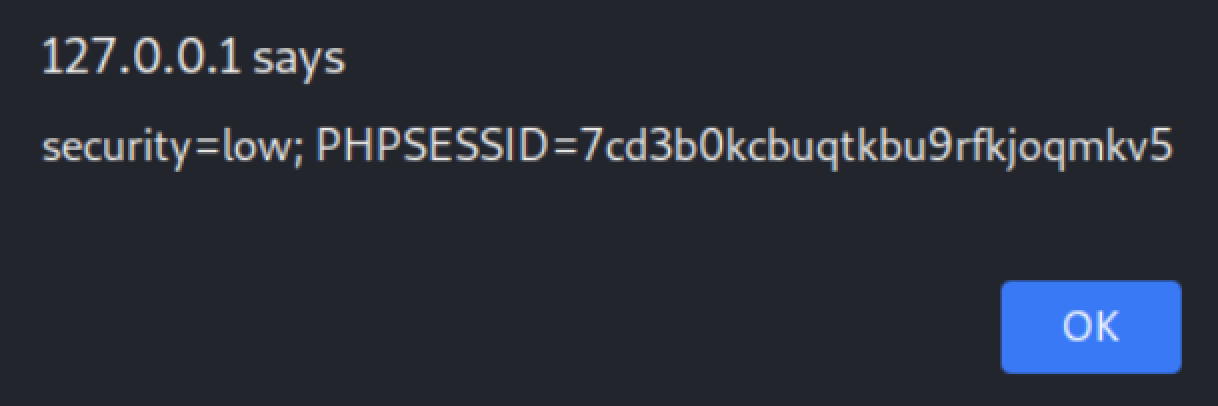
\includegraphics[scale=0.4]{16}
\caption{Site faillible aux attaques CSRF}
\end{figure}
Nous regardons le code source de la page afin de trouver une vulnérabilité. En effet, la page est bien sensible aux attaques de type CSRF. Elle n’est pas protégée par la demande d’une nouvelle authentification au moment de changer le mot de passe, par exemple.
\begin{figure}[H]
\centering
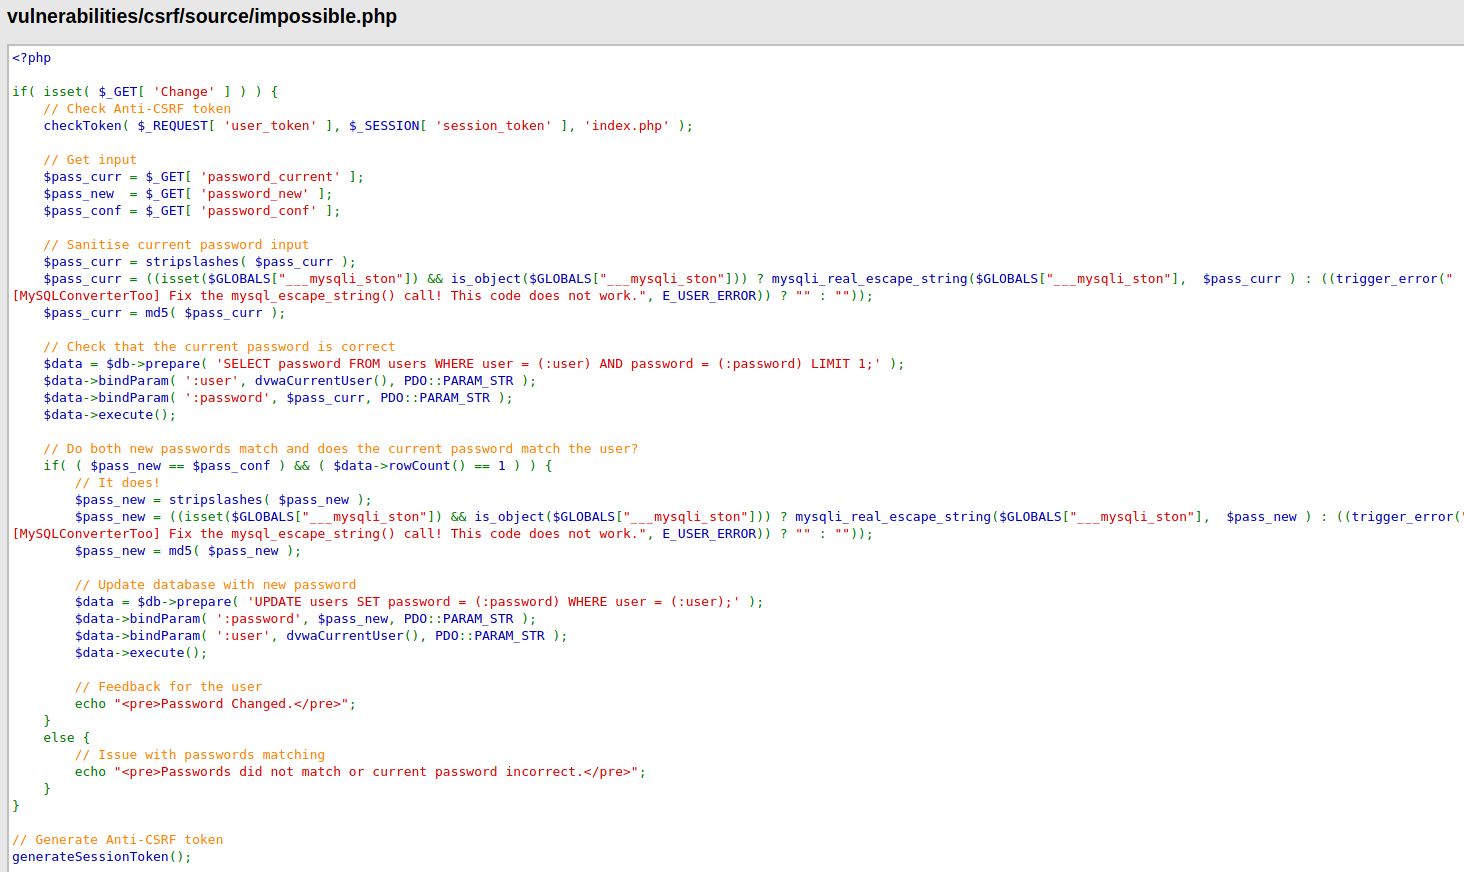
\includegraphics[scale=0.4]{17}
\caption{Code source de la page}
\end{figure}
Nous copions le code source de la page. (Il est possible d’utiliser l’outil httrack)
\begin{figure}[H]
\centering
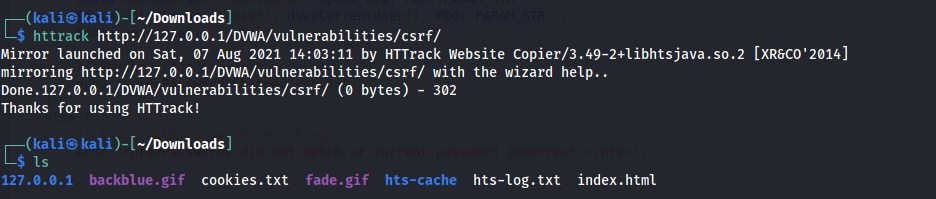
\includegraphics[scale=0.3]{18}
\caption{Copie du code source}
\end{figure}
Nous modifions le formulaire afin de dissimuler les champs password.
\begin{figure}[H]
\centering
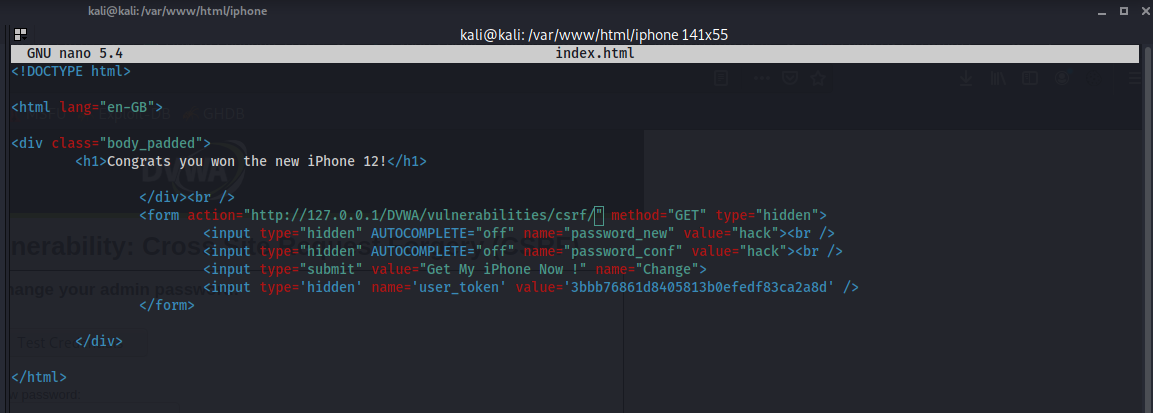
\includegraphics[scale=0.4]{19}
\caption{Modification du code source}
\end{figure}
En cliquant sur le bouton, la victime se voit changer son mot de passe par la valeur “hack” rentrée par défaut.
\begin{figure}[H]
\centering
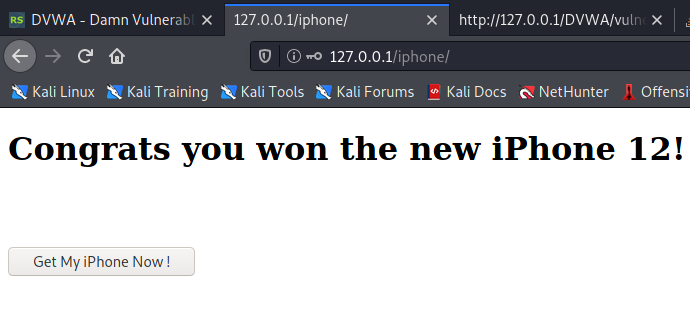
\includegraphics[scale=0.4]{20}
\caption{Exploitation de la faille}
\end{figure}
Le mot de passe de la victime a bien été changé.
\begin{figure}[H]
\centering
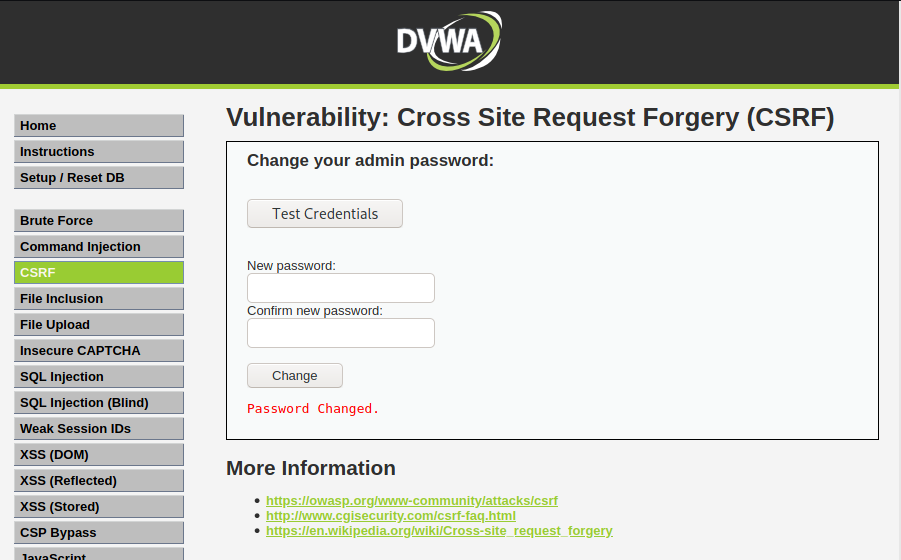
\includegraphics[scale=0.4]{21}
\caption{Mot de passe modifié}
\end{figure}

\end{document}